

\chapter{Detailed proofs of Chapter~\ref{ch:bn_ortho}}


 \section{Preliminaries}
%  \subsection*{Notations}
 Let $v,w \in \R^{k}$ then $v \odot w \in \R^{n}$ with coordinates
 \begin{align}
     [v \odot w ]_{i} = v_i w_i
 \end{align}
 Furthermore $v^{\otimes 2} \in \R^{k \times k}$ with entities
 \begin{align}
     [v^{\otimes 2}]_{ij} = v_i v_j. 
 \end{align}
 In Table~\ref{ortho:tab:notations}, we summarize notations introduced previously. 
 \begin{table}[!ht]
     \centering
     \begin{tabular}{|l|l l|}
     \hline
        Notation & Type & Definition \\ 
        \hline
        $\ell$  & integer & number of layers\\
        $n$  & integer & batch size \\ 
        $d$ & integer & width of the network\\ 
        $k$ & integer & output dimension \\ 
        $X$ & $\R^{d\times n}$ & input matrix\\ 
        $H_\ell$ & $\R^{d\times n}$ & hidden representations at $\ell$ (obeying Eq.~\eqref{ortho:eq:bn_recurrence})\\
        $BN$ & $\R^{d\times n} \to \R^{d\times n}$ & batch normalization layer (defined in Eq.\eqref{ortho:eq:bn_recurrence}) \\ 
        $\text{Law}(X)$ &  & the law of random matrix $X$ \\ 
        $\sigma_i(M)$ & $\R^{k_1\times k_2} \to \R_+$ & the $i$th largest singular value of matrix $M$ \\ 
        $I_k$ & $\R^{k \times k}$ & Identity matrix of size $k$ \\
        $\ones_k$ & $\R^n$ &  all-ones vector
       \\ \hline
     \end{tabular}
     \vspace{0.1cm}
    \caption{Summary of notations used in this chapter.}
     \label{ortho:tab:notations}
 \end{table}
 \subsection*{The Markov chain of hidden representations} Recall the chain of the hidden representations, denoted by $\{ H_\ell\in \R^{d\times n} \}$, obeying the following recurrence: 
 \begin{align} \label{ortho:eq:BNrecurrence_app}
     H_{\ell+1} = \frac{1}{\sqrt{d}}
     BN(W_\ell H_\ell), \quad BN(M) = \left(\diag(M M^\top)\right)^{-\sfrac{1}{2}}M,
 \end{align}
 where $W_\ell \in \R^{d\times n}$ are random weight matrices with i.i.d. zero-mean Gaussian elements. It is easy to check that the Frobenius norm of $H_\ell$ is one due to the row-wise normalization: 
 \begin{equation}
  \label{ortho:eq:unitnorm_app}   
 \begin{aligned} 
    \tr \left(  BN(H) BN(H)^\top \right) & = \tr\left( \diag(H H^\top)^{-\sfrac{1}{2}} H H^\top\diag(H H^\top)^{-\sfrac{1}{2}}\right) \\ 
    & = \tr\left( \diag(H H^\top)^{-1} H H^\top\right) \\ 
    & = d.
 \end{aligned}
 \end{equation}
 \subsection*{Lyapunov function characterizing the orthogonality}
 We introduce the following function serving as a Lyapunov function $\widehat{V}:\R^{d\times n}$ characterizing the orthogonality of the hidden representations:
 \begin{align}
     \widehat{V}(H) = \frac{1}{n} - (\sigma_n (H))^2,
 \end{align}
 where $\sigma_n(H)$ is the minimum singular value of matrix $H$. Next lemma proves $\widehat{V}(H_\ell)$ bounds the orthogonality gap. 
 \begin{lemma} \label{ortho:lemma:Vbound}
 For all hidden representations $H_\ell$, the following holds:
 \begin{align}
     V(H_\ell) \leq 2 n \widehat{V}(H_\ell) \nonumber. 
 \end{align}
 \end{lemma}
 \begin{proof}
 Let $\sigma_1, \dots, \sigma_n$ be the singular values of $H_\ell$. Given these singular values, one can compute $V(H_\ell)$ as 
 \begin{align*}
     (V(H_\ell))^2 = \sum_{i=1}^n \left(\sigma_i^2-\frac{1}{n}\right)^2 \nonumber.
 \end{align*}
 According to Eq.~\eqref{ortho:eq:unitnorm_app}, $\sum_{i=1}^2 \sigma_i^2 = 1$ holds. The proof is an immediate consequence of this propery.   
 \begin{align} \nonumber
     V^2(H_\ell) &=  \sum_{i=1}^n \sigma_i^4 - 2 \underbrace{\left(\sum_{i=1}^n \sigma_i^2  \right)}_{=1}\frac{1}{n} + \frac{1}{n}\\ 
     & = \sum_{i=1}^n \sigma_i^4 -\frac{1}{n}. \nonumber
 \end{align}
 For a freeze $\sigma_n$, the maximum of $\sum_{i=1}^n \sigma_i^4 -\frac{1}{n}$ subject to $\sum_{i=1}^n \sigma_i^2 = 1$ is met when $\sigma_1^2 = 1-(n-1)\sigma_n^2$ and $\sigma_2 = \dots = \sigma_n$.
 Using this optimal values, we get the following bound:
 \begin{align} \nonumber
     V^2(H_\ell) \leq 2(n-1)^2 \underbrace{\left( \frac{1}{n} - \sigma_n^2\right)^2}_{=\widehat{V}^2(H_\ell(X))}.
 \end{align}
 Taking the square root of both sides concludes the proof.
 \end{proof}
 
 
 
 \section{Proof of Theorem~\ref{ortho:thm:contraction}}
 
 The proof of Theorem~\ref{ortho:thm:contraction} relies on the following Theorem that characterizes the change of $\widehat{V}$ in consecutive layers. 
 \begin{theorem} \label{ortho:thm:single_update}
 The sequence $\{ H_\ell \}$ obeys
 \begin{align*}
  \E \left[ \widehat{V}(H_{\ell+1}) | H_\ell \right] \leq \left(1- \frac{2}{3} \left(\frac{1}{n}- \widehat{V}(H_\ell)\right) \right) \widehat{V}(H_\ell) + \frac{1}{\sqrt{d}}.
 \end{align*}
 \end{theorem}
 Notably, the above result does not rely on Assumption \ref{ortho:assume:lineary_indepdence}.  Assuming that  Assumption \ref{ortho:assume:lineary_indepdence} holds, we complete the proof of Theorem~\ref{ortho:thm:contraction}. Combining the last Theorem by this assumption, we get 
 \begin{align} \label{ortho:eq:lyp_condition}
     \E \left[ \widehat{V}(H_{\ell+1}) \right] \leq \left(1-\frac{2}{3}\alpha\right) \E \left[ 
 \widehat{V}(H_\ell)\right] + \frac{1}{\sqrt{d}} 
 \end{align}
 Induction over $\ell$ yields
 \begin{align*}
     \E \left[ \widehat{V}(H_{\ell+1}(X)) \right] & \leq  \left(1-\frac{2}{3}\alpha\right)^{\ell} \E \left[ 
 \widehat{V}(H_1)\right] + \left(\sum_{k=1}^\ell (1-\frac{2}{3}\alpha)^k\right)\frac{1}{\sqrt{d}} \\
     & \leq \left(1-\frac{2}{3}\alpha\right)^{\ell} \E \left[ 
 \widehat{V}(H_1)\right] + \frac{3}{2\alpha\sqrt{d}} 
 \end{align*}
 An application of Lemma~\ref{ortho:lemma:Vbound} completes the proof: 
 \begin{align*}
     \E \left[ V(H_{\ell+1}) \right] & \leq 2 n \E \left[ \widehat{V}(H_{\ell+1}) \right] \\ 
     & \leq 2 \left(1-\frac{2}{3}\alpha\right)^{\ell}+ \frac{3 n}{2 \alpha\sqrt{d}} 
 \end{align*}
 \subsection*{Stability analysis without technical assumption}
 Using Theorem~\ref{ortho:thm:single_update}, we can prove stability of the chain $\{ H_\ell \}$ without Assumption~\ref{ortho:assume:lineary_indepdence}. After rearrangement of terms in Theorem~\ref{ortho:thm:single_update}, we get
 \begin{align*}
     \E \left[ \widehat{V}(H_{\ell+1})| H_\ell \right] - \widehat{V}(H_\ell) \leq - \frac{2}{3} \widehat{V}(H_\ell) \left( \frac{1}{n}- \widehat{V}(H_\ell) \right) + \frac{1}{ \sqrt{d}}
 \end{align*}
 Taking the expectation over $H_\ell$ and average over $\ell$ yields
 \begin{align*}
     \E \left[\frac{1}{\ell}\sum_{k=1}^\ell \widehat{V}(H_k) \left( \frac{1}{n}- \widehat{V}(H_k)\right)\right]  \leq \left(\frac{3 \E \left[ \widehat{V}(H_0) \right]}{2 \ell}\right) +\frac{3}{2 \sqrt{d}}
 \end{align*}
 
 
 \section{Proof of Theorem~\ref{ortho:thm:single_update}}
 \label{ortho:sec:proof_thm}
  
 \subsection*{Spectral decomposition.}
 Consider the SVD decomposition of $H_{\ell}$ as $H_{\ell} = U \diag(\sigma) V^\top$ where $U$ and $V$ are orthogonal matrices. Given this decomposition, we get
 \begin{align} \label{ortho:eq:wh}
     W_{\ell} H_{\ell} = \underbrace{W_{\ell} U}_{W} \diag(\sigma) V^\top 
 \end{align}
 Since $W_{\ell}$ is Gaussian and $U$ is an orthogonal matrix, entities of $W$ are also i.i.d. standard normal. We will repeatedly use the above decomposition in our analyses.
 
 
 \subsection*{Concentration analysis.}
 Consider matrix $C_{\ell+1} := H_{\ell+1}^\top H_{\ell+1}$ whose eigenvalues are $\sigma_1^2, \dots, \sigma_n^2$. The SVD decomposition of $H_\ell$ in Eq.~\eqref{ortho:eq:wh} allows us to write $C_{\ell+1}$ as 
 \begin{align*}
     C_{\ell+1} = \frac{1}{d}\sum_{i=1}^d \left( \frac{w_i \odot \sigma }{\| w_i \odot \sigma \|_2 } \right)^{\otimes 2}
 \end{align*}
 where $w_i \in \R^n$ is the $i$-th row of $W$, and $\sigma \in \R^n$ is the vector of singular values of $H_\ell$. Thus, conditioned on $\sigma$, $C_{\ell+1}$ is an empirical average of i.i.d. random vectors. This allows us to prove that this empirical average is concentrated around its expected value. The next lemma states this concentration. 
 \begin{lemma} \label{ortho:lemma:cov_concentration} 
 The following concentration always holds
 \begin{align*}
      \E_{W_{\ell}} \| C_{\ell+1} - \E_{W_\ell} \left[ C_{\ell+1}
     \right] \|^2 \leq 1/d  
 \end{align*}
 where 
 \begin{align} \label{ortho:eq:pn}
     \E_{W_\ell} \left[ C_{\ell+1}
     \right] = \diag(p_1(\sigma), \dots, p_n(\sigma)), \quad p_i(\sigma) := \E \left[ \frac{\sigma_n^2 w_n^2}{\sum_{k=1}^n \sigma_k^2 w_k^2} \right], \quad w_{i} \stackrel{\text{i.i.d.}}{\sim} \N(0,1)
 \end{align}
 \end{lemma}
 The concentration of $C_{\ell+1}$ allows us to prove that the Lyapunov function $\widehat{V}(H_{\ell+1})$ is concentrated around $1/n-p_n(\sigma)$. 
 \begin{lemma}
 The following holds 
 \label{ortho:lemma:concentration}
 \begin{align*}
  \E_{W_{\ell}} \left[ \left( \widehat{V}(H_{\ell+1}) - (1/n-p_n(\sigma))  \right)^2 \right] \leq \frac{1}{d}
  \end{align*}.
 \end{lemma}
 The last lemma allows us to predict the value of random variable $\widehat{V}(H_{\ell+1})$ by deterministic term $1/n-p_n(\sigma)$. 
 \subsubsection*{Contraction.} 
 The decay in $\widehat{V}(H_{\ell+1})$ with $\ell$ is due to term $1/n-p_n(\sigma)$ in the last lemma. This term is less than (or equal to) $V(H_\ell)$.
 \begin{lemma} \label{ortho:lemma:concentration_center}
 For $p_n(\sigma)$ defined in Eq.~\eqref{ortho:eq:pn}, the following holds:
 \begin{align*}
   \left( \frac{1}{n}- p_n(\sigma) \right) \leq \left(1- \frac{2}{3} \left(\frac{1}{n}- \widehat{V}(H_\ell)\right) \right) \widehat{V}(H_\ell).
 \end{align*}
 \end{lemma}
 Combining the last lemma by Lemma~\ref{ortho:lemma:concentration} concludes the proof of Theorem~\ref{ortho:thm:single_update}: 
 \begin{align} \label{ortho:eq:onestep_result_app}
     \E_{W_\ell} \left[  \widehat{V}(H_{\ell+1}) \right] \leq  \left(1- \frac{2}{3} \left(\frac{1}{n}- \widehat{V}(H_\ell)\right) \right) \widehat{V}(H_\ell) + \frac{1}{\sqrt{d}}.
   \end{align}
 To complete the proof, we prove Lemmas~\ref{ortho:lemma:cov_concentration}, \ref{ortho:lemma:concentration}, and \ref{ortho:lemma:concentration_center}.
 \subsubsection*{Proof of Lemma~\ref{ortho:lemma:cov_concentration}}
 Given the spectral decomposition of $H_{\ell}$ in Eq.~\eqref{ortho:eq:wh}, we compute element $ij$ of $C_{\ell+1}$, which is denoted by $[C_{\ell+1}]_{ij}$:
 \begin{align*}
      [C_{\ell+1}]_{ij} = [A^\top A]_{ij} = \frac{1}{d} \sum_{k=1}^d A_{ki} A_{kj}, \quad A_{ki} = W_{ki} \sigma_i/\sqrt{v_k}
 \end{align*}
 where $v_k = \sum_{m=1}^n W_{km}^2 \sigma_m^2 $. Since $W_{km}$ are zero mean and unit variace, we get
 \begin{align*}
    \E [C_{\ell+1}]_{ij} & = 0 \\
    \E [C_{\ell+1}]_{ij}^2 & = \frac{1}{d^2}\sum_{k=1}^d A_{ki}^2 A_{kj}^2 +  \frac{1}{d^2}\sum_{k,k'}^d \underbrace{\E \left[ A_{ki}^2 A_{kj}^2  A_{k'i}^2 A_{k'j}^2\right]}_{=0} \\ 
    & = \frac{1}{d^2}\sum_{k=1}^d A_{ki}^2 A_{kj}^2 
 \end{align*}
 holds for $i\neq j$.
 By summing up over $i \neq j$, we get 
 \begin{align*}
     \sum_{i \neq j} \E [C_{\ell+1}]_{ij} = \frac{1}{d^2} \left(\sum_{k} \left( \sum_{i} A_{ki}^2 \right)^2 - \sum_{ik} A_{ki}^4\right)
 \end{align*}
 For the diagonal elements, we get 
 \begin{align*}
     \E \left[ C_{\ell+1} \right]_{ii} & = \frac{1}{d}\sum_{k=1}^d \E A_{ki}^2 \\ 
     & = \frac{1}{d}\sum_{k=1}^d \E A_{ki}^2 \\ 
     & = \underbrace{\frac{1}{d}\sum_{k=1}^d \E \left[ \frac{W_{ki}^2 \sigma_i^2 }{\sum_{j=1}^n W_{kj}^2 \sigma_j^2} \right]}_{p_i(\sigma)}
 \end{align*}
 The variance of $[C_{\ell+1}]_{ii}$ is bounded as 
 \begin{align*}
      \text{var}([C_{\ell+1}]_{ii}) & = \E \left(\frac{1}{d}\sum_{k=1}^d (A_{ki}^2 - p_i(\sigma))\right)^2 \\ 
      & = \frac{1}{d^2}\sum_{k=1}^d (A_{ki}^2 - p_i(\sigma))^2 \\
      & \leq \frac{1}{d^2}\sum_{k=1}^d A_{ki}^4 
 \end{align*}
 Combining results for the diagonal and off-diagonal elements yields
 \begin{align*}
     \E \| C_{\ell+1} - \E_{W_{\ell}} \left[ C_{\ell+1} \right] \|_F^2 & = \sum_{ij} \text{var}([C_{\ell+1}]_{ij}) \\
     & \leq  \frac{1}{d^2} \left( \sum_{i} A_{ki}^2 \right)^2 =1/d
 \end{align*}
 \subsection*{Proof of Lemma~\ref{ortho:lemma:concentration}}
 Notably, the eigenvalues of $C_{\ell+1}$ are squared singular values of $H_{\ell+1}$. Let $\lambda_n(C)$ denote the $n$th largest eigenvalue of matrix $C$. 
 \begin{align*}
     \E_{W_{\ell}} \left[ \left( \widehat{V}(C_{\ell+1}) - \left(\frac{1}{n} - p_n(\sigma)\right) \right)^2 \right] & \leq \E_{W_{\ell}} \left[ \left(\lambda_n\left(C_{\ell+1}\right) - \lambda_n\left(\E_{W_{\ell}} \left[ C_{\ell+1} \right]\right) \right)^2\right] \\ 
     & = \E_{W_\ell} \left[ \| C_{\ell+1} - \E_{W_{\ell}} \left[ C_{\ell+1} \right] \|_F^2  \right] \\ 
     & \leq \frac{1}{d}
 \end{align*}
 where the last inequality relies on Lemma~\ref{ortho:lemma:cov_concentration}. 
 \subsubsection*{Proof of Lemma~\ref{ortho:lemma:concentration_center}}
 The proof is based an application of moment generating function that allows us to compute expectations of ratios of random variables. 
 \begin{lemma}[Lemma~1 in ~\citep{sawa1972finite}]
 Let $X_1$ be a random variable that is positive with probability one and $X_2$  be an arbitrary random variable. Suppose that there exists a joint moment generating function of $X_1$ and $X_2$: 
 \begin{align*}
     \phi(\theta_1,\theta_2) = \E \left[ \exp(\theta_1 X_1 + \theta_2 X_2) \right]
 \end{align*}
 for $ \theta_1 \leq \epsilon$ and $| \theta_2 | <\epsilon$ where $\epsilon$ is some positive constant. Then 
 \begin{align*}
     \E \left[ \frac{X_2}{X_1}\right] = \int_{-\infty}^0 \left[\frac{\partial \phi(\theta_1,\theta_2)}{\partial \theta_2} \right]_{\theta_2 = 0 } d \theta_1 
 \end{align*}
 \end{lemma}
 \noindent To estimate $p_n(\sigma)$, we set $X_2 := \sigma_i^2 w_i^2$ and $X_1 = \sum_{j} \sigma_j^2 w_j^2 $, which obtains 
 \begin{align*}
     \phi&(\theta_1,\theta_2) \\
     & = \E \left[ \exp(\theta_1 X_1 + \theta_2 X_2) \right] \nonumber\\ 
     & = (2\pi)^{-n/2}\int_{-\infty}^{\infty}\exp( (\theta_1 + \theta_2) \sigma_i^2 w_i^2 + \sum_{j\neq i} \theta_1 \sigma_j^2 w_j^2) \exp(-\sum_{k} w_k^2/2) d w \\ 
     & = (2\pi)^{-n/2}\int_{-\infty}^{\infty} \exp(\left(-0.5+(\theta_1+\theta_2) \sigma_i^2\right) w_i^2) d w_i  \left(\prod_{j\neq i} \int_{-\infty}^{\infty} \exp(\left(-0.5+\theta_1 \sigma_j^2\right) w_j^2) d w_j\right)\\ 
     & = \frac{1}{\sqrt{1-2 (\theta_1 +  \theta_2)\sigma_i^2}} \left( \prod_{j\neq i} \frac{1}{\sqrt{1-2\theta_1 \sigma_j^2}} \right).
 \end{align*}
 Taking derivative with respect to $\theta_2$ yields 
 \begin{align*}
     \frac{\partial \phi}{\theta_2}(\theta_1,0) = \frac{\sigma_i^2}{(1-2 \theta_1\sigma_i^2)^{3/2}}\left( \prod_{j\neq i} \frac{1}{\sqrt{1-2\theta_1 \sigma_j^2}} \right)
 \end{align*}
 Using the result of the last lemma, we get 
 \begin{align*}
     p_i(\sigma) = \int_{-\infty}^0 \frac{\sigma_i^2}{(1-2 \theta\sigma_i^2)}\left( \prod_{j} \frac{1}{\sqrt{1-2\theta \sigma_j^2}} \right) d\theta
 \end{align*}
 % \paragraph{A sanity check:} It is easy to check that
 % \begin{align}
 %   \frac{\sigma_i^2}{(1-2 \theta\sigma_i^2)}\left( \prod_{j} \frac{1}{\sqrt{1-2\theta \sigma_j^2}} \right) = d\left(\prod_{j} \frac{1}{\sqrt{1-2\theta \sigma_j^2}}\right)/d\theta
 % \end{align}
 % Hence $\sum_{i=1}^p p_i(\sigma) = 1$. \\
 Therefore, 
 \begin{align} \label{ortho:eq:pnbound}
      p_n(\sigma) = \sigma_n^2 f_n(\sigma), \quad f_n(\sigma) :=  \int_{-\infty}^0 \frac{d\theta }{(1-2\theta\sigma_n^2)^{\sfrac{3}{2}}\prod_{j\neq n}(1-2\theta \sigma_j^2)^{\sfrac{1}{2}}} 
  \end{align}
 Since $\sum_{i=1}^n \sigma_i^2 = 1$ holds (see Eq.~\eqref{ortho:eq:unitnorm_app}), $f_n(\sigma)$ in the above formulation is minimized when the $\sigma_j^2$s are all equal for all $j\neq n$. Let $\sigma_n^2:=1/n-\delta$ and $\sigma_j^2:=1/n+\delta/(n-1)$ for all $j\neq i$. This allows us to establish a lowerbound on $f_n(\sigma)$ as
 \begin{align} \label{ortho:eq:g}
 f_n(\sigma) &\ge \int_0^\infty \underbrace{\left(1+2\theta\left(\frac{1}{n}-\delta\right)\right)^{-\frac{3}{2}}\left(1+2\theta\left(\frac{1}{n}+\frac{\delta}{n-1}\right)\right)^{-\frac{n-1}{2}}}_{g(\delta):=} d\theta
 \end{align}
 Next lemma proves that $g(\delta)$ is a convex function for $\delta \in [0,1/n]$. 
 \begin{lemma} \label{ortho:lemma:convexity_g}
   The function $g(\delta)$, which is defined in Eq.~\eqref{ortho:eq:g}, is a convex function on domain $\delta \in [0,1/n]$. 
 \end{lemma}
 The convexity of $g(\delta)$ yields
 \begin{align*}
 g''(\delta)\ge 0\; \forall \delta &\implies g(\delta) \ge g(0) + \delta g'(0)
 \end{align*}
 The above bound allow us to bound $f_n(\sigma)$ as 
 \begin{align*}
     f_n(\sigma)&\ge \int_0^\infty g(0)d\theta + \delta \int_0^\infty 2\theta\left(1+\frac{2\theta}{n}\right)^{-\frac{n}{2}-2} d\theta \\
  &= 1 +\frac{2  \delta n}{n+2}
 \end{align*}
 Note that we use integration by parts to compute the above integrals. 
 Recall $\delta = \frac{1}{n}- \sigma_n^2$.
 Combining the above inequality by Eq.~\eqref{ortho:eq:pnbound} concludes the proof of the Lemma~\ref{ortho:lemma:concentration_center}:
 \begin{align*}
     \frac{1}{n} - p_n(\sigma) \leq \left(1-\frac{2n}{(n+2)}\sigma_n^2\right)\left(\frac{1}{n} - \sigma_n^2\right)
 \end{align*}
 % Notably, the lower-bound is tight for $f_i(\sigma)$ as it is illustrated in the following Figure.
 %  \begin{figure}[!ht]
 %     \centering
 %      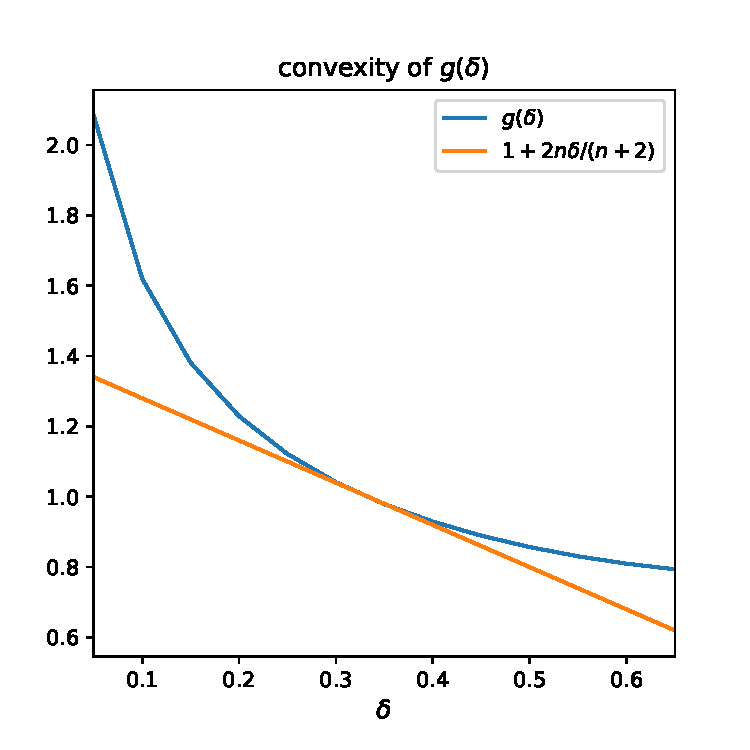
\includegraphics[width=0.4\textwidth]{figures/lemma6_convexity.pdf} 
 % \end{figure}
 \subsubsection*{Proof of Lemma~\ref{ortho:lemma:convexity_g}}
 We can show convexity of $g(\delta)$ by showing $g''(\delta)\ge 0$ for all $\delta\in [0,1/n]$. To this end, 
 we define function $h_1(\delta)$ (for the compactness of notations) as
 \begin{align*}
 h_1(\delta):=\left(1+2\theta\left(\frac{1}{n}-\delta\right)\right)^{-5/2}\left(1+2\theta\left(\frac{1}{n}+\frac{\delta}{n-1}\right)\right)^{-\frac{n-1}{2}-1}.
 \end{align*}
 Given $h_1$, the derivative of $g$ reads as 
 \begin{align*}
 % g(\delta)&:=\left(1+2\theta(\frac{1}{n}-\delta)\right)^{-3/2}\left(1+2\theta(\frac{1}{n}+\frac{\delta}{n-1})\right)\\
 g'(\delta) &=  h_1(\delta)\left( -\frac{3}{2}(-2\theta)\left(1+2\theta\left(\frac{1}{n}+\frac{\delta}{n-1}\right)\right) - \frac{n-1}{2}\left(\frac{2\theta}{n-1}\right) \left(1+2\theta\left(\frac{1}{n}-\delta\right)\right)\right)\\
 &= \theta h_1(\delta) \left(3 + \theta\frac{6}{n} + \theta\delta\frac{6}{n-1}-1-\frac{2 \theta}{n}+2\theta\delta\right)\\
 &= \theta h_1(\delta) \underbrace{\left(2+\theta \frac{4}{n}+\theta\delta\frac{2n+4}{n-1}\right)}_{h_2(\delta):=}\\
 &= \theta h_1(\delta) h_2(\delta).
 \end{align*}
 One can readily check that $h_2'(\delta) \ge 0$. Hence, $h_1'(\delta)\ge 0$ ensures the convexity of $g(\delta)$. Consider the following auxiliary function
 $$h_3(\delta):=\left(1+2\theta\left(\frac{1}{n}-\delta\right)\right)^{-7/2}\left(1+2\theta\left(\frac{1}{n}+\frac{\delta}{n-1}\right)\right)^{-\frac{n-1}{2}-2}.$$
 Given $h_3$, we compute $h'_1$ as 
 \begin{align*}
 h_1'(\delta) &= h_3(\delta)\left(\left(-\frac{5}{2}\right)\left(-2\theta\right)\left(1+2\theta\left(\frac{1}{n}+\frac{\delta}{n-1}\right)\right) + \left(-\frac{n-3}{2}\right)\frac{2\theta}{n-1}\left(1+2\theta\left(\frac{1}{n}-\delta\right)\right)\right)\\
 &= h_3(\delta)\theta\left(5(1+2\theta/n+\frac{2\theta\delta}{n-1}) - \frac{n-3}{n-1}(1+2\theta/n-2\theta\delta)\right)\\
 &=h_3(\delta)\theta\underbrace{\left(\frac{4n-2}{n-1}+2\theta\frac{4n-2}{n(n-1)}+2\theta\delta\frac{n+2}{n-1}\right)}_{h_4(\delta):=}\\
 &=\theta h_3(\delta) h_4(\delta).
 \end{align*}
 Clearly we have $h_3(\delta),h_4(\delta)\ge 0$ for $\delta \in [0,\frac{1}{n}]$. Therefore, the proof is complete.  
 
 
 % \begin{lemma} \label{ortho:lemma:distance_bound}
 %   For $H_{\ell}$ obeying Eq.~\eqref{ortho:eq:bn_recurrence}, the following holds 
 %   \begin{align}
 %       \| [\sigma_1(H_\ell), \dots, \sigma_n(H_{\ell})] - [1/\sqrt{n}, \dots, 1/\sqrt{n}] \|^2_2 \leq n^3 \left( V(H_\ell) \right)^2 
 %   \end{align}
 %  \end{lemma}
%  \subsection*{Results for vanilla networks} \label{ortho:sec:vanilla_theory}
 To compare networks with and without BN,
  next lemma formally establishes the contraction of orthogonality gap to a large value for networks withou BN. 
 \begin{lemma} \label{ortho:lemma:linear}
 Let $S_{\ell} = W_{\ell} \dots W_{1}$. Then, there exists a positive constant $\delta$ such that the following holds
 \begin{align}
       \lim_{\ell \to \infty} \frac{1}{2 \ell}\log\left( \left|V(S_\ell)-\sqrt{\frac{n-1}{n}}\right|\right) \leq -\delta. 
  \end{align}
 \end{lemma} 
 In other words, the gap $V(S_\ell)$ converges to $\sqrt{(n-1)/n}$ with asymptotic rate $\exp(-\delta \ell)$ for the identity inputs. While, Thm.~\ref{ortho:thm:contraction} proves the gap for BN networks converges to $n/\sqrt{d}$ with an exponential rate. For a sufficiently large $d$, $n/\sqrt{d} \ll \sqrt{(n-1)/n}$ holds.
 \begin{proof}
 
 Let $\sigma_1(\ell) \geq \sigma_2(\ell) \geq  \dots \geq  \sigma_n(\ell)$ denote singular values of matrix $S_\ell$, then it is known that 
  \begin{align}
      \lim_{\ell \to \infty} \frac{1}{\ell} \log(\sigma_i^2(\ell)) = \frac{1}{2} \left( \log(2) + \Psi\left(\frac{d-i+1}{2}\right) \right) 
  \end{align}
  holds where $\Psi$ is digamma function~\citep{newman1986distribution}, which a monotonically decreasing function. Therefore, 
  \begin{align} 
       \lim_{\ell \to \infty} \frac{1}{\ell} \left( \log(\sigma_2^2(\ell)) - \log(\sigma^2_1(\ell)) \right)  = - \delta <0 
  \end{align}
  holds for $\delta>0$ that can be exactly computed using function $\Psi$. The above inequality implies that $\sigma_1^2(\ell)$ increases (or decreases) faster than $\sigma_2^2(\ell)$ with an exponential rate. 
  Using this result, we get the following limit for $j\neq 1$:
  \begin{align} \label{ortho:eq:delta_bound1} 
     \lim_{\ell \to \infty} \frac{1}{\ell} \log\left(\frac{\sigma_j^2(\ell)}{\sum_{i} \sigma_i^2(\ell)}\right) \leq \lim_{\ell \to \infty} \frac{1}{\ell} \log\left(\frac{\sigma_2^2(\ell)}{ \sigma_1^2(\ell)}\right) = -\delta
  \end{align}
  Furthermore,
  \begin{align} 
  \label{ortho:eq:delta_bound2}
      \lim_{\ell \to \infty} \frac{1}{2\ell} \log\left|\frac{\sigma_1^2(\ell)}{\sum_{i} \sigma_i^2(\ell)} - 1\right| 
       \leq \lim_{\ell \to \infty} \frac{1}{\ell} \log\left|\frac{n \sigma_2^2(\ell) }{ \sigma_1^2(\ell)}\right| \leq -\delta + \lim_{\ell \to \infty} \log(n)/\ell \leq -\delta 
  \end{align}
  Let $\sigma(\ell) = (\sigma_1^2(\ell), \dots, \sigma_n^2(\ell)) \in \R^n$ and $1_n$ is the all one vector in $\R^n$ and $e_1 = (1,0, \dots, 0)\in \R^n$.
  Using triangular inequality, we get
  \begin{align}
      \left| V(S_\ell) -  \sqrt{(n-1)/n} \right| & = \left|  \left\| \frac{\sigma(\ell)}{\| \sigma(\ell)  \|_1 }- \frac{1}{n} 1_n \right\| - \left\| e_1 -  \frac{1}{n} 1_n  \right\|    \right|  \leq \left\| \frac{\sigma(\ell)}{\| \sigma(\ell)  \|_1} - e_1 \right\| 
  \end{align}
  Therefore, we get
 
   \begin{multline}
      \lim_{\ell \to \infty} \frac{1}{\ell} \log\left( \left|V(S_\ell)-\sqrt{\frac{n-1}{n}}\right|\right) \\ \leq 
      \lim_{\ell \to \infty} \left( \frac{1}{4\ell} \log \left( 2n \left(\frac{\sigma_2^2(\ell)}{\sum_{j} \sigma_j^2(\ell)} \right)  \right) + \frac{1}{4\ell} \log\left(2  \left( \frac{\sigma_1^2(\ell)}{\sum_{j} \sigma_j^2(\ell)} - 1 \right)^2 \right)\right)
   \end{multline}
  which is bounded by $-\delta$ according to the established bounds in Eq.~\eqref{ortho:eq:delta_bound1}, and Eq.~\eqref{ortho:eq:delta_bound2}. 
  \end{proof}
 
\subsection*{Proof of Lemma~\ref{ortho:lemma:wv_bound}}
 The main idea is based on a particular coupling of random matrices $W_\ell H_\ell$ and $G$. Consider the truncated SVD decomposition of $H_\ell$ as $H_\ell = U \diag(\sigma) V^\top $ where $U \in \R^{d\times n}$ and $V \in \R^{n \times n}$ are orthogonal matrices. Due to the orthogonality, the law of $W_\ell U$ is the same as those of $G V $. By coupling $W_\ell U = G V$, we get 
 \begin{equation*}
 \begin{aligned}
     \left(\mathcal{W}_2(W_\ell H_\ell, G/\sqrt{n})\right)^2 & = \inf_{\text{all the couplings}}\E \|   W_\ell U \diag(\sigma) V^\top  - GVV^\top/\sqrt{n} \|_F^2 \\ 
     & \leq \E \| GV \left( \diag(\sigma) - I/\sqrt{n} \right) V^\top \|_F^2 \\ 
     & = \E \tr(GV \left( \diag(\sigma) - I/\sqrt{n} \right) V^\top V \left( \diag(\sigma) - I/\sqrt{n} \right) V^\top G^\top ) \\ 
     & =  \tr(V \left( \diag(\sigma) - I/\sqrt{n} \right) \left( \diag(\sigma) - I/\sqrt{n} \right) V^\top \E \left[ G^\top G \right] ) \\ 
     &= \E \tr( \left( \diag(\sigma) - I/\sqrt{n} \right) \left( \diag(\sigma) - I/\sqrt{n} \right) V^\top V )  \\ 
     &= \E \| \left( \diag(\sigma) - I/\sqrt{n} \right) \|_F^2 \\
     & = \E \left[  \sum_{i=1}^n (\sigma_i -1/\sqrt{n})^2 \right]  \\ 
 &= \E \left[  \sum_{i=1}^n \left(\sigma_i^2 -1/n\right)^2/\left(\sigma_i + 1/\sqrt{n}\right)^2 \right] \\
 & \leq n \E \left[  \sum_{i=1}^n \left(\sigma_i^2 -1/n\right)^2 \right] \\ 
 & \leq n \E \left[ V^2(H_\ell) \right] \\ 
 & \leq 2 n \E \left[ V(H_\ell) \right].
 \end{aligned}
 \end{equation*}
 
 
 \section{Orthogonality gap for the iterative initialization} \label{ortho:sec:init}
 Recall the proposed initialization for weights based on SVD decomposition $H_\ell = U_\ell \Sigma_\ell V_\ell^\top$.
 \begin{align*}
     W_\ell = \frac{1}{\| \Sigma_\ell^{\sfrac{1}{2}}\|_F} V_\ell' \Sigma_\ell^{-\sfrac{1}{2}} U_\ell^\top.
 \end{align*}
 Here, we show that 
 \begin{align}
      V(H_\ell) > V(W_\ell H_\ell) 
 \end{align}
 holds as long as $V(H_\ell) \neq 0$ and \ref{ortho:assume:lineary_indepdence}$(\alpha,\ell)$ holds. 
 Given singular values $H_\ell$, we get 
 \begin{equation}
     \label{ortho:eq:VHell}
     \begin{aligned} 
     V(H_\ell) &= \sum_{i=1}^n \left( \sigma_i^2 - \frac{1}{n}\right)^2 \\ 
     & = \sum_{i} \sigma_i^4 - 1/n, 
 \end{aligned}
 \end{equation}
 where we used $\sum_{i=1}^n \sigma_i^2 = 1$ (see Eq.~\eqref{ortho:sec:perliminaries}).
 Now, we compute $V(H_\ell)$ using the singular values. 
 \begin{align*}
     W_\ell H_\ell = \frac{1}{\| \Sigma_\ell^{\sfrac{1}{2}}\|_F}  V_\ell' \Sigma^{\sfrac{1}{2}}_\ell V_\ell 
 \end{align*}
 Hence, the following holds 
 \begin{align*}
      V(W_\ell H_\ell) & = \sum_{i=1}^n \left( \frac{\sigma_i}{\sum_j \sigma_j} - \frac{1}{n} \right)^2  \\ 
      & = \frac{1}{(\sum_{i=1}^n \sigma_i)^2} - 1/n
 \end{align*}
 Combining with Eq.~\eqref{ortho:eq:VHell}, we get 
 \begin{align*}
     V(H_\ell) - V(W_\ell H_\ell) = \sum_{i=1}^n \sigma_i^4 - \frac{1}{(\sum_{i=1}^n \sigma_i)^2} .
 \end{align*}
 To show that the right side of the above equation is positive, we need to prove  
 \begin{align*}
     \sum_{i} \sigma_i^4 \left(\sum_{i=1}^n \sigma_i\right)^2 > 1 = \left( \sum_{i} \sigma_i^2 \right)^4
 \end{align*}
 holds. Using Cauchy-Schwarz inequality, we get 
 \begin{align*}
     \left( \sum_{i} \sigma_i^2 \right)^4 & = \left( \sum_{i} \sigma_i^{\sfrac{3}{2}} \sigma_i^{\sfrac{1}{2}} \right)^4 \\ 
     & \leq \left( \sum_{i} \sigma_i \right)^2 \left( \sum_{i} \sigma_i^2 \sigma_i \right)^2 \\ 
     & \leq  \left( \sum_{i} \sigma_i \right)^2 \left( \sum_{i} \sigma_i^4 \right),
 \end{align*}
 where the equality in the above inequality is met only for $\sigma_i^2 = \frac{1}{n}$ (so $V(H_\ell) = 0$) under \ref{ortho:assume:lineary_indepdence}. 
 
 
%  \subsection*{Activation functions and the orthogonality} \label{ortho:sec:activations}
%  We have seen hidden representations become increasingly orthogonal through layers of BN MLPs with linear activations. 
%  We observed similar results for MLP with ReLU activations and also a simple convolution network (see Figure~\ref{ortho:fig:relu_convnet}). Here, we elaborate more on the role activation functions in our analysis. 
 
%  \begin{figure}[!ht]
%       \centering
%       \begin{subfigure}[b]{0.4\textwidth}
%           \centering        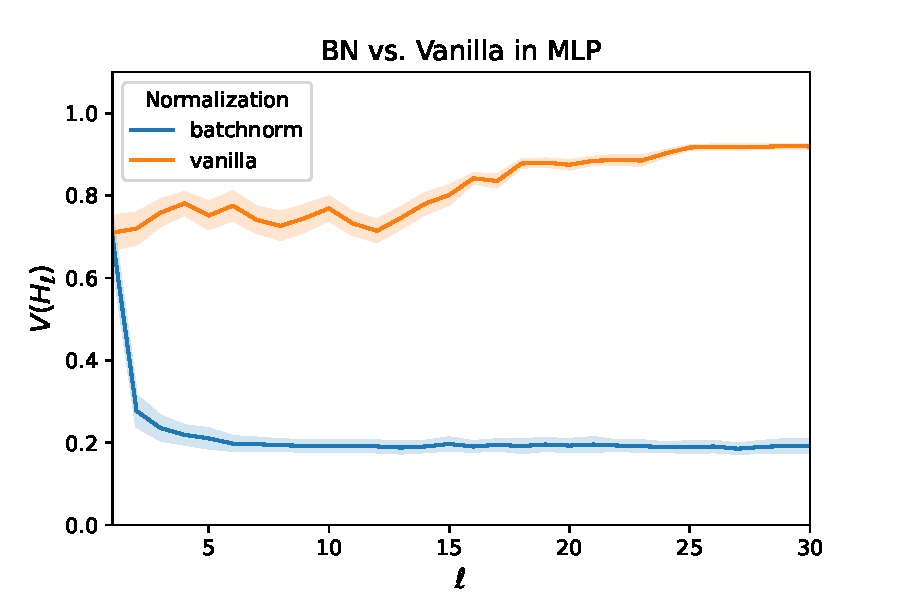
\includegraphics[width=\textwidth]{figures/Fig6A.pdf}
%           \caption{MLP}
%           \label{ortho:fig:relu_mlp}
%       \end{subfigure}
%       \begin{subfigure}[b]{0.4\textwidth}
%           \centering         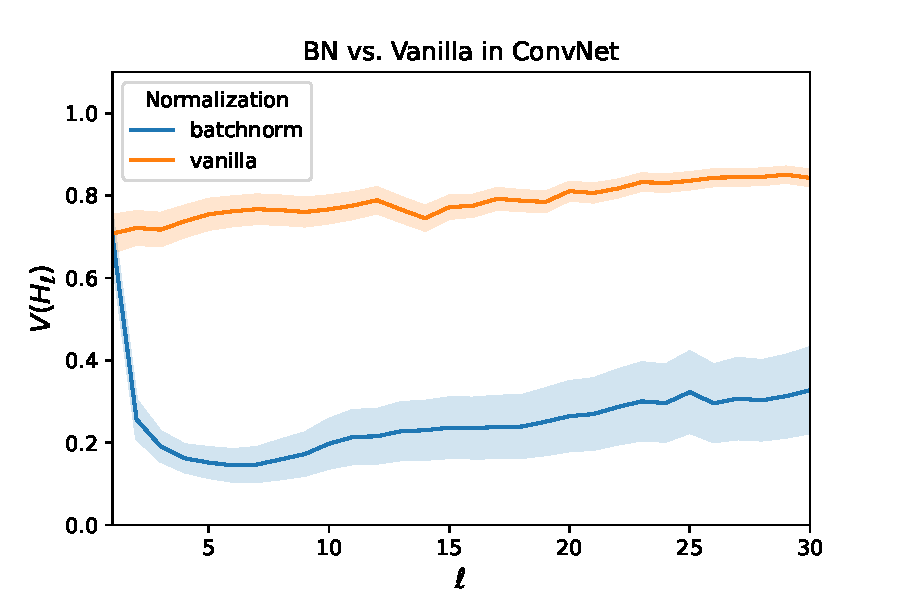
\includegraphics[width=\textwidth]{figures/Fig6B.pdf}
%           \caption{ConvNet}
%           \label{ortho:fig:convnet}
%       \end{subfigure}
%          \caption{Orthogonality gap of layers for BatchNorm vs vanilla network with ReLU, for MLP and a basic convolutional network on CIFAR10. Batch size was set to $8$, the number of hidden layers for both networks was set to $30$, with $100$ width for MLP and $100$ channels for ConvNet in all hidden layers. For the ConvNet, the kernel size was set to $3$, across all hidden layers, with zero-padding to make convolutional feature maps equal sized. The standard deviations were computed for $50$ different randomly sampled batches.}
%          \label{ortho:fig:relu_convnet}
%  \end{figure}
%  For an arbitrary activation function $F$, the hidden representations make the following Markov chain: 
%  \begin{align*}
%      Q_{\ell+1} = BN'(W_\ell F(Q_\ell)).
%  \end{align*}
%  where we assume that $BN'$ makes rows of its input matrix zero-mean and unit variance (the mean correction is included).
%  \subsubsection*{Conjecture}
%  Suppose that $\{ Q_\ell \}$ is \textit{ergodict} \citep{eberle2009markov}, and admits a unique invariant distribution denoted by $\nu$. We define function $L:\R^{d\times n}\to \R_+$ as
%  \begin{align}
%       L(Q_\ell)  = \left\| Q_\ell^\top Q_\ell - \E_{Q\sim \nu} \left[  Q^\top Q \right] \right\|_F .
%  \end{align}
%  We conjecture that there exists an integer $k$ such that for $\ell>k$ the following holds: 
%  \begin{align}
%      \E \left[ L(Q_\ell) \right] =\bigo\left( \frac{1}{ \sqrt{d}} \right).
%  \end{align}
%  Figure~\ref{ortho:fig:activations} experimentally validates that the above result holds for standard activations such as ReLU, sigmoid, and tanh. 
 
%  \begin{figure}[!ht]
%      \centering
%      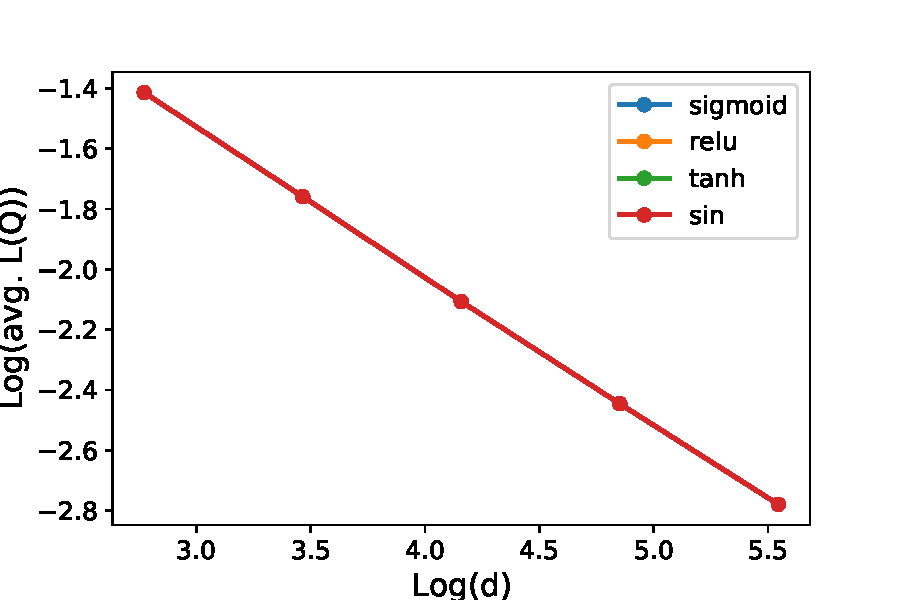
\includegraphics[width=0.45\textwidth]{figures/activations.pdf}
%      \caption{\footnotesize{\textbf{Validating the conjecture.} Horizontal axis: $\log(d)$; vertical axis: $\log(\frac{1}{1000}\sum_{k=1}^{1000} L(Q_k))$. The difference between the plots is negligible, hence not visible. }}
%      \label{ortho:fig:activations}
%  \end{figure}
 
 
 
  
 
%  \subsubsection*{Odd activations}
%  We observe that Theorem~\ref{ortho:thm:contraction} holds for odd activations such as $\sin$ and $\tanh$ with no need to the mean correction in BN. For these activation result of Theorem~\ref{ortho:thm:contraction}. 
%  \begin{align*}
%      \E \left[ V(H_{\ell+1}) \right]  = \bigo\left( (1-\alpha)^{\ell} + \frac{1}{\sqrt{d}}\right) 
%  \end{align*}
%  holds under \ref{ortho:assume:lineary_indepdence}$(\alpha,\ell)$. Remarkably, this is consistent with our conjecture with $ V = L$ for these activations.   



 \section{Comparisons with a BN-replacement}
 \label{ortho:sec:bnreplace}
 Here, we compare iterative orthogonalization with two baselines: (i) initialization with random orthogonal weights \citep{saxe2013exact}, and (ii) adaptive gradient clipping \citep{brock2021high}.
 \begin{itemize}
     \item[(i).] Orthogonal weights achieve orthogonal representations in deep \textit{linear} networks. Consider a MLP whose weight are initialized by Xavier's scheme. Let the weight matrix at layer $\ell$ admit the SVD decomposition $W_\ell = U_\ell \diag(\sigma_\ell) V_\ell$. Then, we replace the weight matrix by the orthogonal matrix $(\text{mean}(\sigma_\ell)) U_\ell V_\ell^\top $. Since ReLU networks with orthogonal weights are prone to the alignment of representations in deep layers, we observed that such an initialization does not help with the slow down of training with depth (see Fig.~\ref{ortho:fig:clipping1}).  
     \item[(ii).] Recently, \cite{brock2021high} propose an effective replacement for BN ---- based on gradient clipping. Let $G_\ell$ denotes the gradient of training loss with respect to $W_\ell$. Given a clipping parameter $\lambda$, adaptive gradient clipping adjusts the norm of $G_\ell$ as
     \begin{align}
         \widehat{G}_\ell = \begin{cases} 
         \left(\lambda \frac{\|W_\ell \|_F^*}{\| G_\ell \|_F}\right) G_\ell & \frac{\| G_\ell \|_F}{\| W_\ell \|_F^*} \geq \lambda \\ 
         G_\ell & \text{otherwise}
         \end{cases}
     \end{align}
     where $\| W_\ell \|_F^* = \max\{\| W_\ell \|_F, 10^{-2} \}$. 
 \end{itemize}
 Fig.~\ref{ortho:fig:clipping1}, and ~\ref{ortho:fig:clipping2} presents results for two different choice of clipping parameters $\lambda=0.1$ and $\lambda=1$, respectively. These plots demonstrate adaptive gradient clipping  effectively alleviates the training slow down with depth. Yet, we observe iterative orthogonalization achieves a better training loss after 30 epochs. 
 It is not known how the clipping enhance the training. While, iterative orthogonalization is inspired by orthogonalization of representations with BN layers, which is theoretically established in this chapter.
 \begin{figure}[!ht]
      \centering
      \begin{subfigure}[b]{0.3\textwidth}
          \centering        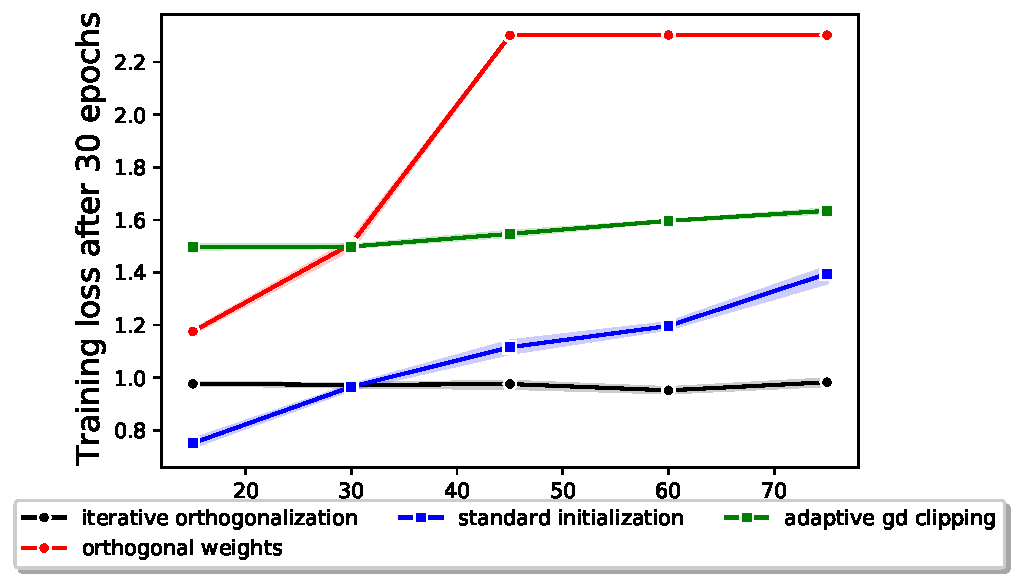
\includegraphics[width=\textwidth]{figures/baselines.pdf}
          \caption{$\lambda=0.1$}
          \label{ortho:fig:clipping1}
      \end{subfigure}
      \begin{subfigure}[b]{0.3\textwidth}
          \centering         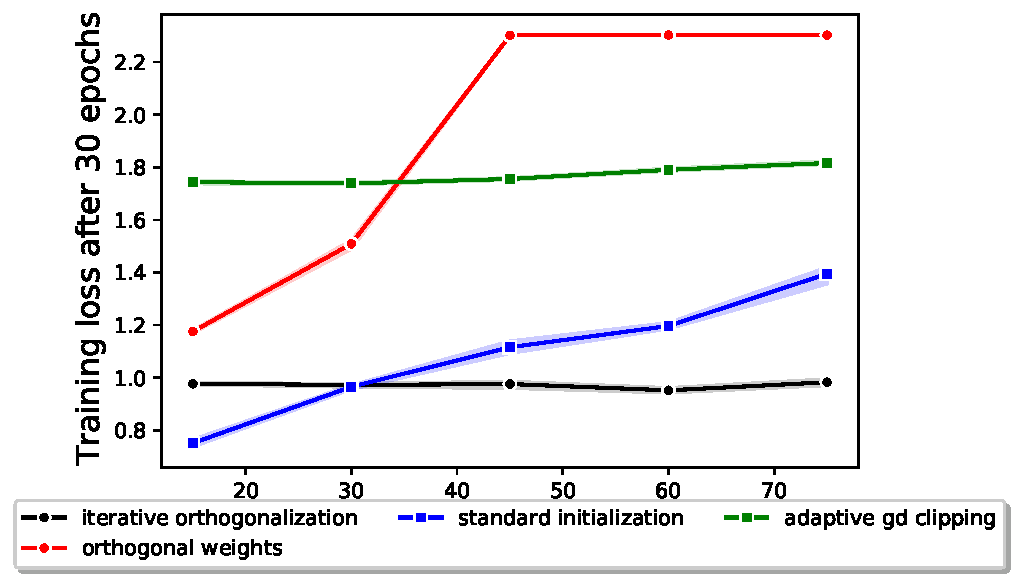
\includegraphics[width=\textwidth]{figures/baselines2.pdf}
      \caption{$\lambda=1$}
  \label{ortho:fig:clipping2}
      \end{subfigure}
         \caption{Iterative orthogonalization vs adaptive gradient clipping. Horizontal axis: the network depth. Vertical axis: training loss for each network after 30 SGD epochs. For more details, see Sec.~\ref{ortho:sec:optimization}.  Mean and 95\% confidence interval of 4 independent runs.}
 \end{figure}


%  \subsection*{Experiments for convolutional networks}
%  \label{ortho:sec:experiments}
%  The introduced initialization scheme in Section~\ref{ortho:sec:optimization} extends to convolutional networks.  In convolutional networks, hidden representation are in the tensor form $H_\ell \in \R^{d\times m \times m \times n}$ where $d$ is the number of filters and $k$ is the image dimensions. Let matrix $W_\ell^{d \times k^2}$ are weights of convolutions layer $\ell$ with kernel size $k$ and $d$ filters.  A 2D convolution is a matrix multiplication combined by a projection as:
%  \begin{align}
%      \text{conv2d}(W_\ell,H_\ell) = \text{fold}\left( W_{\ell} \underbrace{\text{unfold}(H_\ell)}_{H'_\ell}\right)
%  \end{align}
%  where the unfolding extract batches of $k\times k$ from images in tensor $H_\ell$, and folding operation combines the computed convolution for the extracted batches. 
%  We use the SVD decomposition $H'_\ell = U_\ell \Sigma_\ell V_\ell$ to initialize weights $W_\ell$, exactly the same as Eq.~\eqref{ortho:eq:init_w}: 
%  \begin{align*}
%      W_\ell = \frac{1}{\| \Sigma_\ell^{\sfrac{1}{2}}\|_F} V_\ell' \Sigma_\ell^{-\sfrac{1}{2}} U_\ell^\top,
%  \end{align*}
%  where $V_\ell'$ is a slice of $V_\ell$.
%   We experimentally validate the performance of this initialization for two convolution networks with ReLU activations consisting of 20 and 80 convolutions. Table~\ref{ortho:tab:convnet} outlines the details of these neural architectures. 
%  \begin{table}[!ht]
%      \centering
%      \begin{tabular}{|c|c|}
%      \hline
%         The network with 20 layers  &   The network with 80 layers \\
%         \hline
%         Conv2d(3, 64)+    MaxPool2d(2) + RELU 
%         & Conv2d(3, 64)+   MaxPool2d(2) + RELU  \\
%         Conv2d(64, 192) + MaxPool2d(2) + ReLU &  Conv2d(64, 192) + MaxPool2d(2) + ReLU \\
%         Conv2d(192, 256)
%         + Conv2d(256, 256) +ReLU & Conv2d(192, 256)
%          Conv2d(256, 256) + ReLU
%          \\ 
%          \hline 
%          $\{$Conv2d(256, 256)+ReLU$\} \times 16$ &  $\{$Conv2d(256, 256)+ReLU$\} \times 76$
%          \\ 
%          \hline
%          MaxPool2d(2) + ReLU & MaxPool2d(2) + ReLU \\ 
%          Dropout(0.5) + Linear(1024,4096) + ReLU & Dropout(0.5) + Linear(1024,4096) + ReLU \\ 
%          Dropout(0.5) + Linear(4096,4096) + ReLU & Dropout(0.5) + Linear(4096,4096) + ReLU \\ 
%          Linear(4096,10) & Linear(4096,10)
%          \\
%          \hline
%      \end{tabular}
%      \caption{\footnotesize{Convolutional networks used in the experiment.} These neural architectures are obtained by adding layers to AlexNet~\citep{srivastava2014dropout}. The kernel size is 3 for all the convolutional layers. }
%      \label{ortho:tab:convnet}
%  \end{table} 
 
%  \begin{figure}
%      \centering
%      \begin{tabular}{c c}
%          20 layers &  80 layers\\
%         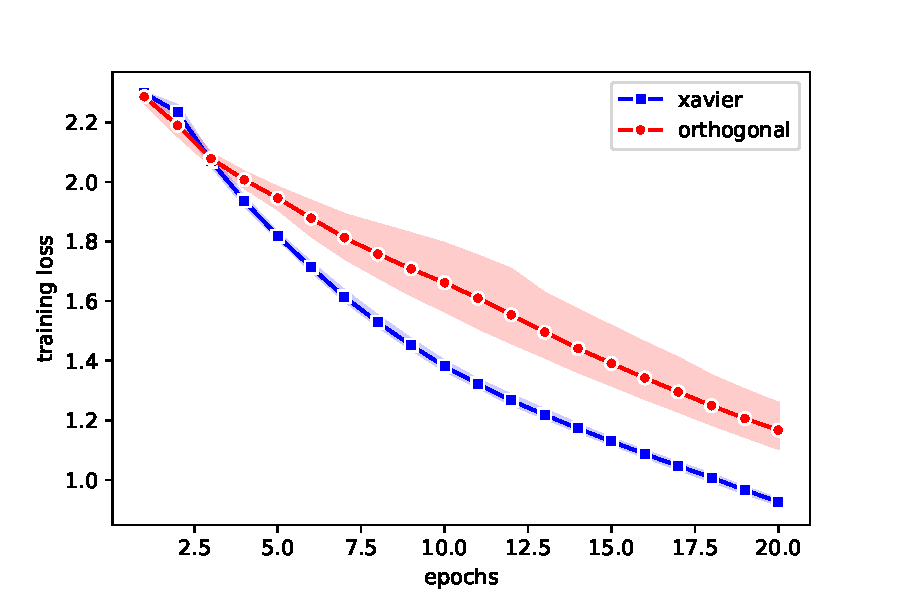
\includegraphics[width=0.4\textwidth]{figures/convolutional_15.pdf}  & 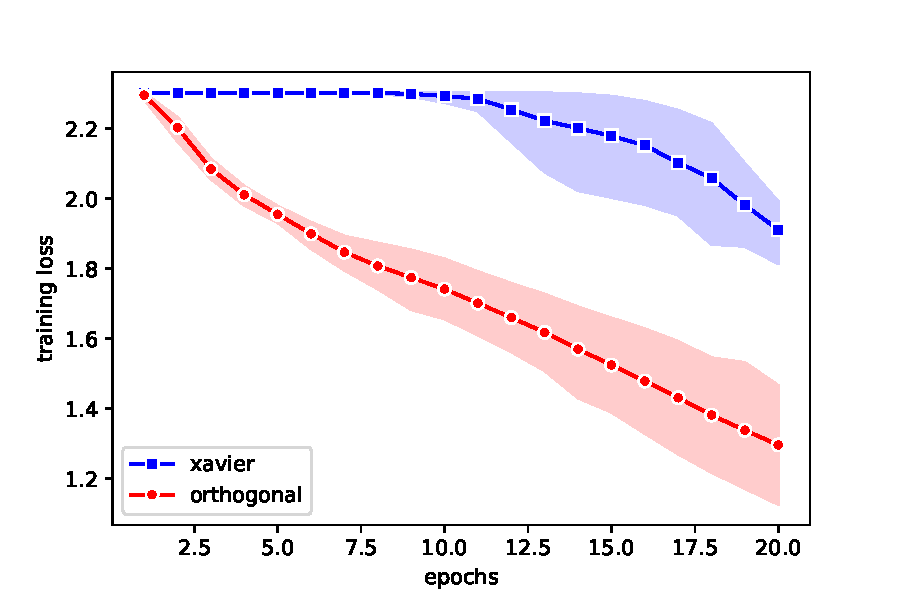
\includegraphics[width=0.4\textwidth]{figures/convolutional_75.pdf}
%      \end{tabular}
%      \caption{\footnotesize{\textbf{Training convolutional networks.} Convergence of SGD for Xavier's initialization \citep{glorot2010understanding} (in blue) and also the proposed initialization method that ensures the orthogonality of hidden representations (in red).  Mean and 95\% confidence interval of 4 independent runs.} }
%      \label{ortho:fig:convents}
%  \end{figure}
 
%  Figure~\ref{ortho:fig:convents} shows the performance of SGD (with stepsize $0.001$ and batchsize 30) for the proposed initialization. This initialization slows SGD for the shallow network with 20 layers compared to standard Xavier's initialization~\citep{glorot2010understanding}. However, it outperforms Xavier's initialization when the depth is significantly large. This result substantiates the role of orthogonality in training. We repeated this experimented for deeper networks and more epochs. Figure~\ref{ortho:fig:conv80} presents our results for a convolutional network with 90 layers and 80 epochs demonstrating orthogonal initialization boosts SGD performance even after many SGD epochs.  
 
 
 
 
%  Although the convolution network used in this experiment is not a conventional network, this experimental result motivates further investigations of the role of orthogonality in standard convolutional networks.
 
%  \begin{figure}
%      \centering
%      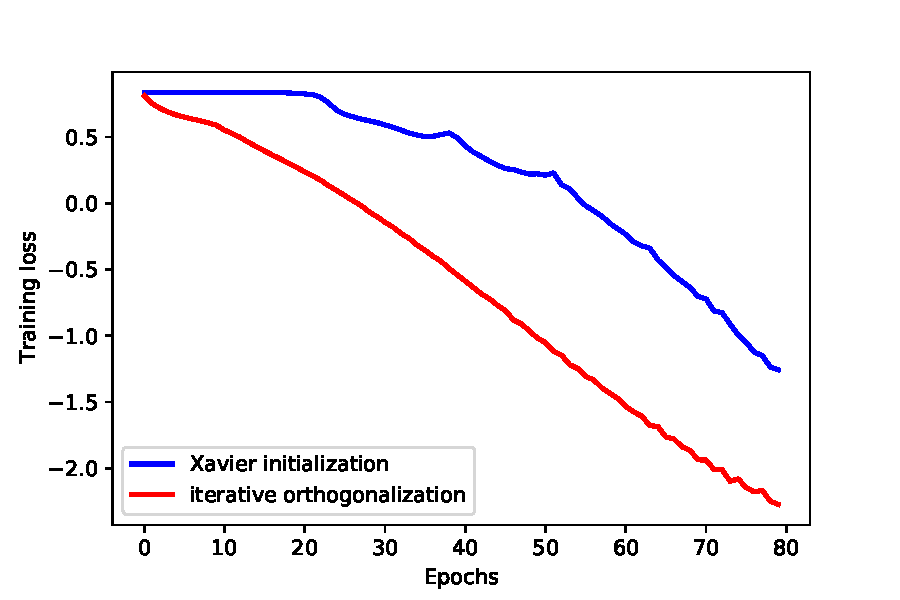
\includegraphics[width=0.5\textwidth]{figures/conv80.pdf}
%      \caption{\footnotesize{\textbf{Training convolutional networks.} Convergence of SGD for Xavier's initialization \citep{glorot2010understanding} (in blue) and also the proposed initialization method that ensures the orthogonality of hidden representations (in red).  Mean of 2 independent runs.} }
%      \label{ortho:fig:conv80}
%  \end{figure}
 
\chapter{Proof of Chapter~\ref{ch:bn_MF}}\label{ch:bn_MF:proofs}


\section{A concentration bound for the empirical covariance matrix}

The following analysis pertains to the deviation between the sample covariance matrix, normalized by the true covariance, and the identity matrix. For a collection of $d$ independent identically distributed \iid samples in $\R^d$, represented as $x_1, x_2, ..., x_d \in \R^n$, the sample covariance matrix $C_d$ is given by:

\begin{equation}
C_d = \frac{1}{d} \sum_{i=1}^{d} x_i x_i^T.
\end{equation}

The true covariance matrix $C$ is defined as the expected outer product of the samples, or:

\begin{align}
C = \mathbb{E}[x_i x_i^T].
\end{align}

We are interested in bounding the deviation of $ C_d$ from the covariance matrix $C$ in terms of their Frobenius norm (denoted as $\|.\|_{F}$), as outlined in the lemma below. Note that if activation $\act$ is uniformly bounded $\act(x)^2\le B x^2,$ and $\BN$ is the batch-norm operator, then ${\|\act(\BN(x))^2\|\le B \|\BN(x)\|^2 \le B n}.$ Thus, activations applied after normalization layers obey the condition of Lemma~\ref{MF:lem:sample_cov_deviation}. With this point in mind, we will prove the concentration result for vectors that are uniformly bounded by the same quantity.


\begin{lemma}\label{MF:lem:sample_cov_deviation}
Let $x_1,\dots,x_d\in \R^n$ be \iid random vectors with covariance $\E x_i x_i^\top = C$ and sample covariance $C_d:=\frac1d \sum_{i=1}^d x_i x_i^\top.$ If the vector norms are universally bounded such that $\norm{x_i}^2\le n \distort  $ holds almost surely, then for $t \lesssim \sqrt{d}$, the following is true:
\begin{align}
P\left(\|C_d - C\|_F \gtrsim t \eps \right) \leq \exp(-t^2), && \eps:=\frac{B n}{\sqrt{d}}.
\end{align}
Here, the probability is taken over the random vectors $x_1,\dots,x_d.$
\end{lemma}

We will use the last lemma to prove Theorem~\ref{MF:thm:concentration}.

\begin{lemma}\label{MF:lem:sample_cov_inv_deviation}
Under the same conditions as Lemma~\ref{MF:lem:sample_cov_deviation}, if the covariance matrix $C$ is not degenerate, i.e., it does not possess zero eigenvalues, for $t \lesssim \sqrt{d}$ it holds
\begin{align}
P\left(\|C^{-1} C_d - I_n\|_F \gtrsim t \eps \right) \leq \exp(-t^2), && \eps:=\frac{B\norm{C^{-1}} n}{\sqrt{d}}.
\end{align}
\end{lemma}

\begin{proof}[Proof of Lemma~\ref{MF:lem:sample_cov_deviation}]
Recall that Bernstein's inequality provides an upper bound on the probability that the sum exceeds a certain threshold $t$. Given \iid variables $X_1,\dots,X_d,$ it states that are uniformly bounded $|X_i|\le B$ for all $i$, we have
\begin{align}
\P\left(\frac{1}{d} \sum_{i=1}^{d} X_i\geq t\right) \leq 2 \exp\left(-\frac{dt^2/2}{K^2 + Kt/3}\right),
\end{align}
where $t > 0$ and $\sigma^2$ is the variance of $\sum_{i=1}^{d} E[ X_i^2] \le d B^2 $. 
Define $X_i:=\|x_i x_i^\top - C\|_F^2.$ We have
\begin{align}
    \|x_i x_i^\top - C\|_F^2 &\le \|x_i x_i\|_F + \|C\|_F\\
    &\le B n + \|E x_i x_i^\top \|_F\\
    &\le B n + E \|x_ix_i\|_F\\
    &\le 2 B n.
\end{align}
% \end{align}
Thus, we can plug $K:= 2 B n $ into the Bernstein's inequality to get 
\begin{align}
&\P\left(\frac1d\sum_{i=1}^{d} \|x_i x_i^\top - C\|_F \geq t\right) \leq\\
&\qquad \exp\left(-\frac{dt^2/2}{ 4 n^2\distort^2 + 2\distort n t/3}\right).
\end{align}
Since $\|\cdot\|_F $ is convex, Jensen's inequality which implies that moving the averaging inside can only decrease its value, which in turn implies 
\begin{align}
&\P\left(\|\frac1d\sum_{i=1}^{d}  x_i x_i^\top - C\|_F \geq t\right)\\
&\qquad \leq \exp\left(-\frac{d t^2}{ 8 n^2\distort^2 (1 + \frac{t}{6n\distort})}\right).
\end{align}
We can now rename $t \sqrt{d}/(\sqrt{8} B n)$ as $t$ and use definition of sample covariance to conclude 
\begin{align}
    \P\left(\|C_d - C\|_F \ge t \frac{\sqrt{8} B n}{\sqrt{d}}\right)\le \exp\left(- \frac{t^2}{(1+\frac{t}{3\sqrt{2 d}})}\right),
\end{align}
which can be restated as
\begin{align}
 \P\left(\|C_d - C\|_F \gtrsim t \eps\right)\le \exp(- t^2), &&  \eps:=\frac{ B n}{\sqrt{d}},
\end{align}
which holds if $t \lesssim \sqrt{d}.$
\end{proof}


\begin{proof}[Proof of Lemma~\ref{MF:lem:sample_cov_inv_deviation}]
Consider transformed vectors $z_i:=C^{-1/2} x_i.$ Note that we have $\E z_i z_i^\top = C^{-1} C = I_n.$ Thus, we can apply Lemma~\ref{MF:lem:sample_cov_deviation} on deviations of sample covariance of $z_i$'s from $I_n.$ Furthermore, we have $\norm{z_i}^2 \le \norm{C^{-1}} \norm{x_i}^2 \le \norm{C^{-1}} B n.$ So we can invoke Lemma~\ref{MF:lem:sample_cov_deviation} by setting $B$ to $\norm{C^{-1}}B .$
\end{proof}

\section{Analyzing Gram Dynamics Around Fixed Points}

Equipped  with the results established so far, we now turn our attention to the dynamics of Gram matrices in relation to the total variation of the Multi-Layer Perceptron (MLP) Markov chain. In particular, we demonstrate a specific construction based on fixed-point $G_*,$ and show that after one layer update the total variation distance is bounded.

% Recall the fixed point $\C$, $T$ in Equation \eqref{MF:eq:dist_recurrence}. Given a random representation $ h\in\R^{d\times n}$ drawn from $h\sim \mu$ \textcolor{blue}{what is $\mu$? shouldn't be $\mu_*$} and Gaussian weights $W\in\R^{d\times d}$ drawn \iid from $\Normal(0,1/d)$, the distribution of $h':=W \act(\BN(h))$ can be obtained by applying the Markov transition to $\mu_{h'}=T(\mu)$. The following Lemma bounds the $tv(h,h')$, thereby proving that the distribution $h$ is almost an invariant distribution for wide neural networks. 

\begin{lemma}[Restated Lemma~\ref{MF:lem:tv_one_step}]\label{MF:lem:one_step_restated}
    Let $\hat h\in\R^{d\times n}$ be constructed by drawing its rows \iid from $\Normal(0,G_*)$. Let $\hat\mu$ denote the distribution of $\hat h$. Given that fixed-point Gram matrix $G_*$ is non-degenerate and the activation is uniformly bounded $\act(x)^2 \le B x^2$, then
    \begin{align}
        \norm{\hat\mu - T(\hat \mu)}_{tv} \lesssim \eps^2 \LN(1/\eps), && \eps:=\frac{n\norm{G_*^{-1}}\distort }{\sqrt{d}},
    \end{align}
    holds if $B$ and $\norm{G_*^{-1}}$ are non-zero. 
\end{lemma}


Under the assumption of geometric contraction, irrespective of the initial distribution, the total variation distance to the stationary distribution contracts by $1-\alpha$, for some $\alpha>0$, after one transition $T$. This result, together with Lemma~\ref{MF:lem:tv_one_step}, provides a tool to approximate the stationary distribution by a matrix constructed from the fixed-point Gram matrix $G_*$.

\begin{lemma}\label{MF:lem:stationary_dist_approximation}
    Let $\hat\mu$ denote the distribution of a random matrix in $\R^{d\times n}$, whose rows are drawn \iid from $\Normal(0,G_*)$. Assuming the rapid mixing condition~\ref{MF:ass:rapid_mixing} holds with constant $\alpha> 0$, then
    \begin{align}
        \norm{\hat\mu-\mu_*}_{tv}\lesssim \alpha^{-1}\eps^2\LN(1/\eps), && \eps:=\frac{n\distort \norm{G^{-1}_*}}{\sqrt{d}}.
    \end{align}
\end{lemma}

We can finally the results about total variation into the context of Gram matrix dynamics through depth.
\begin{lemma}\label{MF:lem:multiple_steps_total_variation}
    Let $\mu_\ell$ denote the hidden representation of a BN-MLP, and $\hat\mu$ denote the distribution of a matrix whose rows are drawn from $\Normal(0,G_*)$. If hidden representations obey the rapidly mixing assumption with rate $1-\alpha,$ for $\alpha>0,$ then 
    \begin{align}
        \norm{\mu_\ell-\hat\mu}_{tv}\lesssim (1-\alpha)^\ell + \alpha^{-1}\eps^2\LN(1/\eps), && \eps:=\frac{n\distort\norm{G_*^{-1}}}{\sqrt{d}}.
    \end{align}
\end{lemma}





With the necessary lemmas in place, we are now ready to present our main theorem.

\begin{theorem}[Restated Theorem~\ref{MF:thm:concentration}]\label{MF:thm:concentration_restated}
For an MLP chain $G_\ell$ that originates from a non-degenerate input $G_0,$ and that has a non-degenerate fixed point $G_,$ and that obeys the rapidly mixing assumption with $\alpha>0,$ we have the following:
\begin{align}
    &\P(\|G_* - G \|_F \ge t)\lesssim \nonumber\\
    &\qquad t^{-2}(\|G_*\|^2 (1-\alpha)^\ell + \alpha^{-1} \eps^2 \LN(1/\eps)),
\end{align}
with $\eps:= n B \kappa(G_*)/\sqrt{d}.$ 
\end{theorem}

The proof of the theorem relies on the following lemma bounds Gram matrix deviations by total variation.

\begin{lemma}\label{MF:lem:total_variation_lower_bound}
Conditioned on Gram matrices $G_*,G\in\R^{n\times n},$ construct $h, \hat h\in\R^{d\times n}$ by drawing their rows \iid from $\Normal(0,G)$ and $\Normal(0,G_*).$ If $G_*$ is non-degenerate, the following hols for total variation between $h$ and $\hat h$:
\begin{align}
    \TV(h,\hat h)\ge \frac{t}{100}\P(\|G_*^{-1} G - I_n\|_F^2 \ge t),
\end{align}
where the probability is defined over $G.$
\end{lemma}

The proof of this theorem follows directly from the lemmas we have established. 

\begin{proof}[Proof of Theorem~\ref{MF:thm:concentration_restated}]
We apply the total variation bound established in Lemma~\ref{MF:lem:multiple_steps_total_variation} and combine this with the lower bound stated in Lemma~\ref{MF:lem:total_variation_lower_bound} 
\begin{align}
    &\frac{t}{100}\P(\|G_*^{-1} G - I_n\|_F^2 \ge t)\\
    &\qquad \le \TV(h_\ell,\hat h)\lesssim (1-\alpha)^\ell + \alpha^{-1} \eps^2 \LN(1/\eps) .\label{MF:eq:main_inequality}
\end{align}
Omitting constants we have
\begin{align}
    &\P(\|G_*^{-1} G - I_n\|_F \ge \sqrt{t})\\
    &\quad \qquad \lesssim t^{-1}((1-\alpha)^\ell + \alpha^{-1} \eps^2 \LN(1/\eps)).
\end{align}
By a change of variables we get
\begin{align}
    &\P\left(\|G_*^{-1} G - I_n\|_F \ge t\right)\\
    &\qquad \lesssim t^{-2}((1-\alpha)^\ell + \alpha^{-1} \eps^2 \LN(1/\eps)).
\end{align}
Note that $\|G^* - G \|_F = \|G^*(G^{-1}_* G - I_n)\|_F,$ which is bounded by $\|G_*\|\|G^{-1}_* G- I_n\|_F.$ Thus
\begin{align}
    &\P\left(\|G_* - G \|_F \ge t\right) \\
    &\quad \le \P\left(\|G_*^{-1} G - I_n\|_F \ge t/\|G_*\|\right) \\
    &\quad \le t^{-2} \|G_*\|^2 ((1-\alpha)^\ell+ \alpha^{-1}\eps^2\LN(1/\eps)),
\end{align}
where the last equation is due to \eqref{MF:eq:main_inequality}. The above inequality obtains
\begin{align}
& \eps:=\frac{ B n }{\sqrt{d}}\|G_*\|\|G_*^{-1}\|\\
  &  \P(\|G_* - G\|_F \ge t)\lesssim \\
  &\qquad \qquad t^{-2}\left( \|G_*\|^2 (1-\alpha)^\ell + \alpha^{-1}\eps^2\LN(1/\eps))\right).
\end{align}
Recall that $\|G_*\|\|G_*^{-1}\|$ encodes the ratio of largest to smallest eigenvalue of $G_*,$ which is its condition number $\kappa(G_*).$ This finalizes the proof. 
\end{proof}


% \begin{proof}
%     We can invoke the total variation bound of Lemma~\ref{MF:lem:multiple_steps_total_variation} and leverage the lower bound of total variation by deviation from identity in Lemma~\ref{MF:lem:total_variation_lower_bound} to conclude the proof. 
% \end{proof}



\begin{proof}[Proof of Lemma~\ref{MF:lem:multiple_steps_total_variation}]
First, note that geometric contraction assumption implies
\begin{equation}
    \tv{\ell}{*}\le (1-\alpha)\tv{\ell-1}{*} \le (1-\alpha)^\ell,
\end{equation}
which by numerical inequality $1-x\le \exp(-x)$ can be bounded by $\exp(-\alpha \ell).$ We can invoke Lemma~\ref{MF:lem:stationary_dist_approximation} and triangle inequality for total variation to conclude the proof.
\end{proof}

\begin{proof}[Proof of Lemma~\ref{MF:lem:stationary_dist_approximation}] 
Recall that the rapidly mixing assumption implies that $\norm{T(\hat\mu)-\mu_*}_{tv}\le (1-\alpha) \norm{\hat\mu-\mu_*}_{tv}.$ Furthermore, invoking Lemma~\ref{MF:lem:one_step_restated}, we have 
\begin{align}
    \norm{T(\hat\mu)-\hat\mu}_{tv}\lesssim \eps^2\LN(1/\eps),\\
  \implies  \norm{\hat\mu-\mu_*}_{tv}\lesssim \alpha^{-1} \eps^2\LN(1/\eps),
\end{align}
where the last line is implied by the triangle inequality for total variation.
\end{proof}


\begin{proof}[Proof of Lemma~\ref{MF:lem:one_step_restated}]
Let us explicitly construct $T(\hat \mu).$ Recall that $\hat\mu$ describes distribution of $\hat h$ whose rows are drawn \iid from $\Normal(0,G_*).$ Define $h:=W \act(\BN(\hat h)),$ where $W$ is a Gaussian with \iid elements $\Normal(0,1/d).$ Thus, by construction, distribution of $h$ follows $T(\hat \mu).$ Our main proof strategy of upper bounding total variation between $\hat h$ and $h$ is to bound it conditioned on the proximity of $G$ to $G_*.$ 

\textbf{Bounding deviations $\|G_*^{-1} G - I\|_F$.}
Recall that based on the fixed-point property of $G_*$ we have 
\begin{align}
    \E_{w\sim N(0,G_*)} \act(\BN(w))^{\otimes 2} = G_*.
\end{align}
Define sampled Gram of activations $G:= \frac1d \act(\BN(\hat h))^\top \act(\BN(\hat h)),$ which is equal in expectation to $\E G = G_*.$ By construction of batch norm operator which maps every row to $\sqrt{n}$-sphere, and the uniform bound $\act(x) ^ 2 \le B x^2, $ we can conclude that rows of $\act(\BN(\hat h))$ are always bounded by 
\begin{align}
    &\|\BN(x)\| \le \sqrt{n} && \forall x\in\R^n\\
  \implies  &\|\act(\BN(x))\| \le \sqrt{B n }, && \forall x\in\R^n\\
  \implies  &\|\row_k(\act(\BN(\hat h)))\|^2 \le B n, && \forall k.
\end{align}
This allows us to invoke Lemma~\ref{MF:lem:sample_cov_inv_deviation} to conclude:
\begin{align}
    \P(\|G_*^{-1} G - I_n\|_F \ge t\eps ) \le \exp(-t^2),
\end{align}
where $\eps = B \|G_*^{-1}\| n/\sqrt{d}.$ 


\textbf{Bounding total variation $\TV(h,\hat h).$} Define set of matrices $N_t:=\{M\in\R^{n\times n}: \norm{\C^{-1}M- I_n}_F^2\le \eps^2 t^2 \}.$ 
% Define Gram matrix $G :=\frac1d \act(\BN(h))\act(\BN(h))^\top$. 
Observe that conditioned on $G$, $h$ is equal in distribution to a matrix rows are drawn \iid from $\Normal(0,G)$. Thus, we can decompose the total variation based on depending on $G$ belonging to neighborhood of $G_*$ or not 
\begin{align}
    \TV(h, \hat h)
    &\le \Prob{\norm{\C^{-1}\Csa-I_n}_F^2 \ge t^2\eps^2 } \\
    & \qquad +  \sup_{G\in N_t}\TV(\Normal(0,G),\Normal(0,G_*))\\
    & \lesssim \Prob{\norm{\C^{-1}\Csa-I_n}_F \ge t\eps} + \frac{3}{2}t^2 \eps^2 ,
\end{align}
where in the last line we use the upper bound on total variation between two Gaussian matrices from~\cite{devroye2018total}. Plugging our result for deviation of $G$ and $G_*$ we have
\begin{align}
    \TV(h, \hat h)\le \frac{3}{2}t^2 \eps^2 + \exp(-t^2),
\end{align}
which holds for all $t \lesssim \sqrt{d}.$ In particular, we can set $t^2:=\LN(2/3\eps^2)$ which implies
\begin{align}
    \TV(h, \hat h) \lesssim \frac{3\eps^2}{2}(1+\LN(2/2\eps^2)),
\end{align}
which omitting constants can be restated as 
\begin{align}
    \TV(h, \hat h) \lesssim \eps^2\LN(1/\eps^2).
\end{align}
To finish the proof, observe that condition $t\lesssim \sqrt{d}$ translates to $\LN(1/\eps^2)=O(d)$ which in turn requires $\eps \gtrsim \exp(-d/2).$ Plugging the definition of $\eps$ we have $n B \|G_*^{-1}\|\gtrsim \sqrt{d} \exp(-d/2).$ Since the right-hand side is $o(1),$ and $n\ge 1,$ this condition will always hold if the boundedness and conditioning are non-zero $B,\| G_*^{-1}\| > 0.$
% By a change of variable and omitting the absolute constants, we have
% \begin{align}
%     \norm{\hat\mu - T(\hat\mu)}_{tv} &\lesssim \eps\LN(1/\eps), && \eps:=\frac{n\distort\norm{G_*^{-1}}}{\sqrt{d}}.
% \end{align}
% Finally, recall the condition for $t/n\distort\le 3/4$, which is equivalent to $\eps \lesssim n\distort ,$ which holds for $\epsilon \lesssim 1.$ For $\eps > 1,$ since the total variation distance is always bounded by $1,$ the inequality becomes vacuous and always true. Thus, the inequality holds for arbitrary $\eps>0.$
\end{proof}


\begin{proof}[Proof of Lemma~\ref{MF:lem:total_variation_lower_bound}]
Define set of matrices $N_t:=\{M\in\R^{n\times n}: \norm{\C^{-1}M- I_n}_F^2\le t \}$. We have
\begin{align}
    \TV(h,\hat h) &= \int_G \P(G)\TV(\Normal(0,G),\Normal(0,G_*)) \\
    & = \int_{G\in N_t} \P(G)\TV(\Normal(0,G),\Normal(0,G_*)) \\
    &\qquad + \int_{G\notin N_t} \P(G)\TV(\Normal(0,G),\Normal(0,G_*)) \\
    &\ge \int_{G\notin N_t} \P(G)\TV(\Normal(0,G),\Normal(0,G_*)) \\
    &\ge \P(G \notin N_t) \inf_{G\notin N_t}\TV(\Normal(0,G),\Normal(0,G_*))\\
    &\ge \frac{t}{100} \P\left(\norm{G_*^{-1}G-I_n}_F^2\ge t\right),
\end{align}
where in the last line we have used the lower bound for total variation of multivariate Gaussians from~\cite{devroye2018total}.
\end{proof}

\chapter{Supplemental proofs and experiments for Chapter~\ref{ch:bn_grad}}




\section{Conditional orthogonalization}
% \input{sections/appendices/conditional_orthogonalization}
\paragraph{Isometry after rotation.}
Our analysis is based on ~\citep[Corollary 3]{joudaki2023impact}, which we restate in the following Lemma:
\begin{lemma}
    \label{grad:lem:isobn}
    For all non-degenerate matrices $X \in \R^{d \times d}$, we have:
    \begin{align}
        \I(\BN(X))\geq \left(1+ \frac{\text{variance}\{\|X_{j\cdot}\|\}_{j=1}^d}{(\text{mean} \{\|X_{j\cdot}\|\}_{j=1}^d)^2}\right) \I(X)~.
    \end{align}
\end{lemma}

Lemma~\ref{grad:lem:isobn} proves isometry bias of $\BN$. The next lemma proves that isometry does not change under rotation  

\begin{lemma}[Isometry after rotation]
% \label{grad:lem:iso_rotation}
Let $X \in \R^{d\times d}$ and $W \sim \mathbb{O}_d$ be a random orthogonal matrix and $X'= W X$. Then,  
\begin{align}
   \I(\BN(X'))\geq \left(1+ \frac{\text{variance}\{\|X'_{j\cdot}\|\}_{j=1}^d}{(\text{mean} \{\|X'_{j\cdot}\|\}_{j=1}^d)^2}\right) \I(X)~.
\end{align}
\end{lemma}
%
\begin{proof}
   Using properties of the determinant, we have 
   \begin{align}
       \det(X' X'^\top ) = \det(W)^2 \det(XX^\top) =  \det(XX^\top),
   \end{align}
   where the last equation holds since $W$ is an orthogonal matrix. Furthermore, 
   \begin{align}
    \tr(X' X'^\top) & = \tr(W X X^\top W^\top ) \\
    & = \tr(XX^\top \underbrace{W^\top W}_{=I}) \\
    & = \tr(XX^\top)~.
   \end{align}
Combining the last two equations with Lemma~\ref{grad:lem:isobn} concludes the proof.
\end{proof}

\paragraph{Increasing isometry with rotations and $\BN$.}
The last lemma proves the isometry bias does not decrease with rotation and $\BN$. However, this does not prove a strict decrease in isometry with $\BN$ and rotation. The next lemma proves there exists an orthogonal matrix for which the isometry is strictly increasing. 
\begin{corollary}[Increasing isometry]
\label{grad:cor:isometry_increase}
Let $X \in \R^{d\times d}$ and denote its singular value decomposition $X = U \diag\left(\{\sigma_i\}_{i=1}^d\right) V^\top$, where $U$ and $V$ are orthogonal matrices. Then, we have:
\begin{align}
    \I (\BN(U^\top H)) = 1~.
\end{align}
\end{corollary}
%
\begin{proof} 
Let $S = \diag \left(\{\sigma_i\}_{i=1}^d \right)$ be the diagonal matrix containing the singular values of $X$. Then, we have:
\begin{align}
    \BN(U^\top X) &= \BN(U^\top U S V^\top) \\
    &= \BN(S V^\top) \\
    &= \diag(SV^\top V S)^{-\frac{1}{2}} SV^\top \\
    &= S^{-1} S V^\top \\
    &= V^\top,
\end{align}
which has maximum isometry 1 since it's an orthonormal matrix.
\end{proof}

Thus, there exists a rotation that increases isometry with $\BN$ for each non-orthogonal matrix.
 The proof of the last corollary is based on a straightforward application of Lemma~\ref{grad:lem:iso_rotation}.



\paragraph{Orthogonalization with randomness.}
The isometric is non-decreasing in Lemma~\ref{grad:lem:iso_rotation} and provably increases for a certain rotation matrix (as stated in the last corollary). Hence, it is possible to increase isometry with random orthogonal matrices. 

\begin{theorem}
    % \label{grad:thm:iso_bound}
    Suppose $W \sim \mathbb{O}_d$ is a matrix drawn from $\mathbb{O}_d$ such that $W\stackrel{d}{=} WU$ for all orthogonal matrices $U$. Let $\{\lambda_i\}_{i=1}^d$ be the eigenvalues of $XX^\top$. Then,
    \begin{align}
        \E_W \left[\I(\BN(WX))\right | X] \geq \left( \frac{1}{ 1 - \frac{\sum_{k=1}^d (\lambda_k - 1)^2}{2d^2(d+2)} } \right) \I(X)   
    \end{align}
    holds for all $X = \BN(\cdot)$, with equality for orthogonal matrices.
\end{theorem}
\begin{remark}
    Note that the assumption on $X=\BN(\cdot),$ can be viewed as an induction hypothesis, in that we can recursively apply this theorem to arrive at a quantitative rate at depth. 
\end{remark}
Notably, $\sum_{i=1}^d \lambda_i = d$ if $X = \BN(\cdot)$. Hence, one can expect that $\sum_{i=1}^d \lambda_i^2 < d^2$ for all full random matrices $X$ in form of $X = \BN(\cdot)$. 

\begin{proof}
We need to compute the variance/mean ratio in Lemma~\ref{grad:lem:iso_rotation}.
Let $X \in \R^{d \times d}$ have SVD decomposition $X = U \diag\{\sigma_i\}_{i=1}^d V^\top$ where $U$ and $V$ are orthogonal matrix and $\sigma_i^2 = \lambda_i$. Since the distribution of $W$ is invariant to transformations with orthogonal matrices, the distribution of $W$ equates those of $X' = W \diag\{\sigma_i\} V^\top$. It easy to check that 
\begin{align}
    \| X_{j\cdot}' \| = \sqrt{\sum_{i=1}^d \sigma_i^2 W_{ji}^2 } = \sqrt{\sum_{i=1}^d \lambda_i W_{ji}^2 }~.
\end{align}
Thus, 
\begin{align}
    \sum_{j=1}^d \| X_{j\cdot}' \|^2 = \sum_{i=1}^d \lambda_i = d, 
\end{align}
where the last equality holds due to the batch normalization.
Thus, we have
\begin{equation}
   \label{grad:eq:proof_iso_bound_eq1}
   \E \left[ \frac{d\sum_{j=1}^d \|X'_{j \cdot} \|^2}{(\sum_{j=1}^d \| X'_{j \cdot} \|)^2} \right] 
   = \E \left[\frac{d^2}{(\sum_j \| X'_{j \cdot} \|)^2} \right] 
   \geq \frac{d^2}{\E \left[ \left(\sum_{j=1}^d \| X'_{j \cdot} \|\right)^2 \right]}~.
\end{equation}
We need to estimate 
\begin{align}
    \E \left[ \| X_i'\| \| X_j'\| \right] = \E \left[ \left(\sum_{k=1}^d \lambda_k W_{ik}^2\right)^{\frac{1}{2}} \left(\sum_{k=1}^d \lambda_k W_{jk}^2\right)^{\frac{1}{2}}\right]~. 
\end{align}
Since square root function is concave, we have $\sqrt{x} \leq 1 + \frac{1}{2} (x-1)$.
Thus 
\begin{align}
    \E \left[\| X'_i \| \| X'_j\| \right]
& \leq \E \left[\left(1 + 0.5 \sum_{k=1}^d (\lambda_k-1) W_{ik}^2 \right) \left(1 + 0.5 \sum_{k=1}^d (\lambda_k-1) W_{jk}^2\right)\right] \\ 
& = 1 + \frac{1}{4} \sum_{k, q} (\lambda_k-1)(\lambda_q -1) \E \left[W_{ik}^2 W_{jq}^2 \right] \\
&= 1 + \frac{1}{4}\left[ \sum_{k \neq q} (\lambda_k-1)(\lambda_q -1)\underbrace{\E \left[ W_{ik}^2 W_{jq}^2 \right]}_{E_1} + \sum_{k=q} (\lambda_k-1)(\lambda_k -1)\underbrace{\E \left[ W_{ik}^2 W_{jk}^2 \right]}_{E_2} \right],
\end{align}
where in the first equality we have used the fact that the cross terms reduce, where the expectations are applications of Weingarten calculus:
\begin{align}
    \E \left[ 0.5 \sum_{k=1}^d(\lambda_k - 1)W_{ik}^2 + 0.5 \sum_{k=1}^d(\lambda_k - 1)W_{jk}^2 \right]
    &= \E \left[ 0.5 \sum_{k=1}^d \lambda_k W_{ik}^2  + 0.5 \sum_{k=1}^d \lambda_k W_{jk}^2 - 1 \right] \\
    &= 0.5 \sum_{k=1}^d \lambda_k \E \left[W_{ik}^2 \right] + 0.5 \sum_{k=1}^d \lambda_k \E \left[W_{jk}^2 \right] - 1 \\
    &= \frac{0.5}{d} \sum_{k=1}^d \lambda_k  + \frac{0.5}{d} \sum_{k=1}^d \lambda_k - 1 \\
    &= 0~.
\end{align}

The main quantity we must compute is an expectation of polynomials taken over the Haar measure of the Orthogonal group $O(n)$. To carry out the computation, we make use of Weingarten calculus~\citep{banica2011polynomial, collins2006integration, weingarten1978asymptotic}. More specifically, we make use of the of the Weingarten formula, studied by~\cite{collins2006integration, collins2022weingarten}:
\begin{align}
    \int_{O(n)} r_{i_1 j_1} r_{i_2 j_2} \dots r_{i_{2d} j_{2d}} d\mu(O(n)) = \sum_{\sigma \in \mathcal{M}_{2d}} \sum_{\sigma \in \mathcal{M}_{2n}} \Delta_\sigma(\boldsymbol{i}) \Delta_\sigma(\boldsymbol{j}) \wg^O(\sigma^{-1}\tau),
\end{align}
where $\mu(O(n))$ is the Haar measure of Orthogonal group. For an in depth explanation of each quantity in the Weingarten formula, we refer the reader to  \citet[Section 5.2]{collins2022weingarten}.

The quantity we focus on is $\E_W \left[W_{ik} W_{ik} W_{jq} W_{jq}\right]$. We will do the computation on multiple cases, based on the equalities of $k, q$. Notice that $i \neq j$ in all cases. It suffices if we focus on the two distinct cases: $E_1 = \E_W \left[W_{ik}^2  W_{jq}^2\right]$ $(k \neq q)$ and $E_2 = \E_W \left[W_{ik}^2  W_{jk}^2\right]$ $(k = q)$.

% We rewrite the expression as $\E_W \left[W_{i \alpha}^2 W_{j \beta}^2 \right] = \E_W \left[W_{i \alpha} W_{i \alpha} W_{j \beta} W_{j \beta} \right]$, where $\alpha, \beta$ will be replaced by all combinations of the indices.

We first compute $E_1$.

Following the procedure from \citet[Section 5.2]{collins2022weingarten}, we take the index sequences to be $\boldsymbol{i} = (i, i, j, j)$ and $\boldsymbol{j} = (k, k, q, q)$. Similarly, we get $\Delta_\sigma(\boldsymbol{i}) = \Delta_{\tau}(\boldsymbol{j}) = 1$ only if $\sigma = \{ \{1, 2\}, \{3, 4\} \}$ and $\tau = \{ \{1, 2\}, \{3, 4\} \}$. 

Consdering $\sigma, \tau$ as permutations, we get:
\begin{align}
    \sigma &= \begin{pmatrix}
                1 & 2 & 3 & 4\\
                1 & 2 & 3 & 4
                \end{pmatrix},  \\
    \tau &= \begin{pmatrix}
                1 & 2 & 3 & 4\\
                1 & 2 & 3 & 4
                \end{pmatrix}, \\
    \sigma^{-1} \tau &= \begin{pmatrix}
                1 & 2 & 3 & 4\\
                1 & 2 & 3 & 4
                \end{pmatrix},
\end{align}
where $\sigma^{-1} \tau$ has coset-type $[1, 1]$. Finally, we plug the results back into the formula and we obtain:
\[
    E_1 = \E_W \left[W_{ik}^2 W_{jq}^2 \right] 
    = \wg^O([1, 1]) 
    = \frac{d+1}{d(d+2)(d-1)},
\]
where the last equality is based on the results in Section 7 of~\cite{collins2009some}.

We compute $E_2$.

Similar to the previous expression, we take the index sequences to be to be $\boldsymbol{i} = (i, i, j, j)$ and $\boldsymbol{j} = (k, k, k, k)$. Thus, we obtain $\Delta_\sigma(\boldsymbol{i}) = \Delta_{\tau}(\boldsymbol{j}) = 1$ only if $\sigma = \{ \{1, 2\}, \{3, 4\} \}$ and $\tau_1 = \{ \{1, 2\}, \{3, 4\} \}$, $\tau_2 = \{ \{1, 3\}, \{2, 4\} \}$, $\tau_1 = \{ \{1, 4\}, \{2, 3\} \}$. Similarly, we compute $\sigma^{-1} \tau_i$ for $i \in \{1,2,3\}$. Notice that $\sigma$ is the identity permutation, thus yielding $\sigma^{-1} \tau_i = \tau_i$, with the coset-types $[1, 1], [2], [2]$ respectively, for each $i \in \{1, 2, 3\}$.

Plugging back into the original equation, we obtain:
\begin{align}
    E_2 = \E_W \left[W_{ik}^2 W_{jk}^2 \right] 
    &= \wg^O([1, 1]) + 2 \wg^O([2]) \\ 
    &= \frac{d+1}{d(d+2)(d-1)} + 2 \frac{-1}{d(d+2)(d-1)} \\
    &= \frac{d-1}{d(d+2)(d-1)}~.
\end{align}

Thus, plugging back into the original inequality, we obtain:
\begin{align}
    \E &\| X'_i \| \| X'_j\| \\
    &\leq 1+\frac{1}{4} \left[ \sum_{k \neq q} (\lambda_k-1)(\lambda_q -1) \frac{d+1}{d(d+2)(d-1)} + \sum_{k=q} (\lambda_k-1)(\lambda_k-1) \frac{d-1}{d(d+2)(d-1)} \right] \\
    &= 1+\frac{1}{4d(d+2)(d-1)} \left[ \underbrace{\sum_{k \neq q} (\lambda_k-1)(\lambda_q -1)}_{S_{\neq}} - \underbrace{\sum_{k=q} (\lambda_k-1)(\lambda_k-1)}_{S_=} \right] \\
    &= 1 - \frac{\sum_k(\lambda_k - 1)^2}{2d(d+2)(d-1)},
\end{align}
where we have used that $S_{\neq} + S_= = \sum_{k,q}(\lambda_k-1)(\lambda_q -1) = (\sum_{k=1}^d (\lambda_k-1))^2=0$ in the last equality.

Thus, we obtain:
\begin{align}
    \E \left[ \left(\sum_j \| X'_{j\cdot} \| \right)^2 \right]
    &= \E \left[ \sum_j \| X_{j\cdot}' \|^2 + 2 \sum_{i < j} \| X'_{i\cdot} \| \| X'_{j\cdot} \| \right] \\
    &= d + 2 \sum_{i < j} \E \left[ \| X'_{i\cdot} \| \| X'_{j\cdot} \| \right] \\
    &\leq d + (d^2 - d)\left( 1 - \frac{\sum_k(\lambda_k - 1)^2}{2d(d+2)(d-1)} \right) \\
    &= d^2 - \frac{\sum_k(\lambda_k - 1)^2}{2(d+2)} \label{grad:eq:bound}~.
\end{align}
\end{proof}

\begin{corollary}[Isometry gap bound]
\label{grad:cor:isogap_bound}
Suppose the same setup as in Theorem~\ref{grad:thm:iso_bound}. Then, we have:
\begin{align}
    \E_W[\psi(X') | X] \leq \psi(X) + \log \left(1 - \frac{\sum_k(\lambda_k - 1)^2}{2d^2(d+2)}\right).
\end{align}
\begin{remark}
    Notice that the term $\frac{\sum_{k=1}^d (\lambda_k - 1)^2}{2d^2(d+2)} = \mathcal{O}(\frac{1}{d})$, yielding $\log\left[1 - \frac{\sum_{k=1}^d (\lambda_k - 1)^2}{2d^2(d+2)} \right] \leq 0$.
\end{remark}
\end{corollary}
%
\begin{proof}
    From Lemma~\ref{grad:lem:iso_rotation}, we know that:
        \begin{align}
            -\log\I(\BN(X')) &\leq -\log\I(X) - \log\frac{d^2}{\left(\sum_{j=1}^d \| X_{j\cdot}' \|\right)^2} \\
            \implies  -\log\I(\BN(X')) &\leq -\log\I(X) - \log{d^2} + \log \left(\sum_{j=1}^d \| X_{j\cdot}' \|\right)^2 \\
            \implies \E_W[-\log\I(\BN(X')) | X] 
            &\leq -\log\I(X) - \log{d^2} + \E_W\left[ \log \left(\sum_{j=1}^d \| X_{j\cdot}' \|\right)^2  \Bigg| X \right] \\
            &\leq -\log\I(X) - \log{d^2} + \log \E_W \left[ \left(\sum_{j=1}^d \| X_{j\cdot}' \|\right)^2 \Bigg| X \right] \label{grad:eq:jensen} \\
            &\leq -\log\I(X) - \log{d^2} + \log \left(d^2 - \frac{\sum_k(\lambda_k - 1)^2}{2(d+2)}\right) \label{grad:eq:prev_bound} \\
            &\leq -\log\I(X) + \log \left(1 - \frac{\sum_k(\lambda_k - 1)^2}{2d^2(d+2)} \right),
        \end{align}
    where in inequality~\ref{grad:eq:jensen} we have used the fact that $\E [\log X] \leq \log \E[X]$ and in inequality~\ref{grad:eq:prev_bound} we have used the bound obtained in proof Theorem~\ref{grad:thm:iso_bound}, equation~\ref{grad:eq:bound}.
    Thus, we obtain:
    \begin{align}
        \E_W[\psi(X') | X] \leq \psi(X) + \log \left(1 - \frac{\sum_k(\lambda_k - 1)^2}{2d^2(d+2)}\right)~.
    \end{align}
\end{proof}

\label{grad:sec:conditional_orthonality}

\section{Isometry gap decay rate}
\label{grad:sec:proof_isometry_depth}
Before we start with the main part of our analysis, let us establish a simple result on the relation between isometry gap and orthogonality: 
\begin{lemma}[Isometry gap and orthogonality]\label{grad:lem:isogap_ortho}
    If $\psi(X)\le \frac{c}{16d},$ then eigenvalues of $X^\top X$ are within $[1-c, 1+c].$
\end{lemma}

Note that, in order to simplify the calculations, we use the fact that $\frac{1}{d(d+2)} \approx \frac{1}{d^2}$ in the following proofs.

Based on the conditional expectation in Corollary~\ref{grad:cor:isogap_bound}, we have:
\begin{align}
    \E \left[\psi(X^{\ell+1}) | X^\ell \right] \le \psi(X^\ell) - \frac{\EV(X^\ell)}{2d^2}~.
\end{align}
Now, we prove a lemma that is conditioned on the previous layer isometry gap being smaller or larger than $\frac{1}{16d}$.
\begin{lemma}[Isometry gap conditional bound]
\label{grad:lem:iso_gap_step_conditional}
    For $X^\ell$ being the representations of an MLP under our setting, we have:
    \begin{align}
    \E \left[\psi(X^{\ell+1}) \middle| X_\ell, \psi(X^\ell) \le \frac{1}{16d}\right] &\le \psi(X^\ell)\left(1-\frac{1}{2d^2}\right), \label{grad:eqn:ineq1} \\
    \E \left[\psi(X^{\ell+1}) \middle| X_\ell, \psi(X^\ell) > \frac{1}{16d}\right] &\le \psi(X^\ell) - \frac{1}{32d^3}~. \label{grad:eqn:ineq2}
    \end{align}
\end{lemma}

\begin{proof}[Proof of Lemma~\ref{grad:lem:iso_gap_step_conditional}]
Let $\lambda_k = 1+\epsilon_k$, and assume without loss of generality that $\sum_{k=1}^d\epsilon_k = 0$. Then, using the numerical inequality $\log(1+x) \ge x - x^2$, when $|x|\le \frac12$ we have:
\begin{align}
&\EV(X) = \frac1d\sum_{k=1}^d\epsilon_k^2\\
&\max_k |\epsilon_k|\le \frac12 \implies \psi(X) = -\frac1d\sum_{k=1}^d\log(1+\epsilon_k) \le -\frac1d\sum_{k=1}^d (\epsilon_k - \epsilon_k^2) = \EV(X)~.
\end{align}
Altogether, we have
\begin{align}
\max_i |\epsilon_i| \le \frac12 \implies \psi(X) \le \EV(X)~.
\end{align}
Now, we can restate the condition in terms of an inequality on the isometry gap. Thus, we can write:


\begin{align}
d\psi(X) = -\sum_{i=1}^d\log\lambda_i = -\sum_{i=1}^d \log(1+\epsilon_i) \ge -\sum_{i=1}^d \left(\epsilon_i - \frac{3\epsilon_i^2}{6+4\epsilon_i}\right) = \sum_{i=1}^d \frac{3\epsilon_i^2}{6+4\epsilon_i},
\end{align}
where we used the fact that $\sum_i\lambda_i = d$ implying $\sum_i\epsilon_i = 0$ and also used the inequality $\log(1+x) \le x-\frac{6+x}{6+4x}$ when $x\ge -1$ for $\epsilon_i$'s. Note that because $|\eps_i| \leq \frac{1}{2}$, we get $6 + 4\epsilon_i \ge 4,$ all terms on the right-hand side are positive, implying that each term is bounded by the upper bound:
\begin{align}
\frac{3\epsilon_i^2}{6+4\epsilon_i}\le d\psi(X) \quad \forall i \in \{1, 2, \dots, d\}~.
\end{align} 

By construction, we have $\epsilon_i\ge -1$ and $\frac{3\epsilon_i^2}{6+4\epsilon_i} \le \frac{1}{16}.$ Since $6+4\epsilon_i \ge 2$, we can multiply both sides by $6+4\epsilon_i$ and conclude $3\epsilon_i^2 - \frac{6+4\epsilon_i}{16} \le 0$. We can now solve the quadratic equation and obtain $\frac{1 - \sqrt{74}}{24} \le \epsilon_i \le \frac{1 + \sqrt{74}}{24}$ which numerically becomes $-0.35\le \epsilon_i \le 0.4$, implying $|\epsilon_i|< 0.5$.

By solving the quadratic equation above we can guarantee that 
\begin{equation}
\label{grad:eq:proof_iso_gap_step_conditional_eq1}
\psi(X)\le \frac{1}{16d} \implies \max_i|\epsilon_i| \le \frac12 \implies \psi(X) \le \EV(X)~.
\end{equation}

Furthermore, we can restate the condition on maximum using: 
\begin{align}
\max_k|\epsilon_k| = \sqrt{\max_k\epsilon_k^2} \le \sqrt{\sum_k\epsilon_k^2} = \sqrt{d\EV(X)}
\end{align}
and conclude that 
\begin{align}
\EV(X) \le \frac{1}{4d} \implies  \max_i |\eps_i|\le \frac12\implies \psi(X)\le \EV(X)~.
\end{align}

Using this statement, we have 
\begin{align}
    \EV(X) \leq \frac{1}{16d} \implies \psi(X)\le \EV(X) \implies \psi(X) \leq \frac{1}{16d}~.
\end{align}
If we negate and flip the two sides we arrive at 
\begin{equation}
\label{grad:eq:proof_iso_gap_step_conditional_eq2}
   \psi(X) > \frac{1}{16d} \implies \EV(X) > \frac{1}{16d}~.
\end{equation}

Thus, we can simplify the recurrence 
\begin{align}
    \E[\psi(X^{\ell+1}) | X^\ell] \le \psi(X^\ell) - \frac{\EV(X^\ell)}{2d^2} 
\end{align}
as follows
\begin{align}
\E\left[\psi(X^{\ell+1}) \middle| X^\ell, \psi(X^\ell) \le \frac{1}{16d}\right] &\le \psi(X^\ell)\left(1-\frac{1}{2d^2}\right),\\
\E\left[\psi(X^{\ell+1}) \middle| X^\ell, \psi(X^\ell) > \frac{1}{16d}\right] &\le \psi(X^\ell) - \frac{1}{32d^3},
\end{align}
where we used \eqref{grad:eq:proof_iso_gap_step_conditional_eq1} in the first one and \eqref{grad:eq:proof_iso_gap_step_conditional_eq2} in the second one.
\end{proof}

\begin{proof}[Proof of Theorem~\ref{grad:thm:iso_gap_decay_in_depth}]
    From Lemma~\ref{grad:lem:isobn}, we know that $\psi(X^0) \geq \psi(X^1) \geq \dots \geq \psi(X^L) \geq 0$, for any layer $0 \leq \ell \leq L$. Thus, we get using~\eqref{grad:eqn:ineq2}:
    \begin{align}
    \E\left[\psi(X^{\ell+1}) \middle| X^\ell, \psi(X^\ell) > \frac{1}{16d}\right] &\leq \psi(X^\ell) - \frac{1}{32d^3} \\
    &= \left(1 - \frac{1}{32d^3\psi(X^\ell)}\right) \psi(X^\ell) \\
    &\leq \left(1 - \frac{1}{32d^3\psi(X^0)}\right) \psi(X^\ell),
    \end{align}    
    where in the last step we have used the fact that $\psi(X^\ell) \leq \psi(X^0)$.

    Thus, we can combine~\eqref{grad:eqn:ineq1} and~\eqref{grad:eqn:ineq2} and obtain:
    \begin{align}
        \E[\psi(X^{\ell+1}) | X^\ell] 
        &= \E\left[\psi(X^{\ell+1}) \middle| X^\ell, \psi(X^\ell) \leq \frac{1}{16d}\right] \1_{\psi(X^\ell) \leq \frac{1}{16d}} \\
        &+ \E\left[\psi(X^{\ell+1}) \middle| X^\ell, \psi(X^\ell) > \frac{1}{16d}\right] \1_{\psi(X^\ell) > \frac{1}{16d}} \\
        &\leq \max\left(\E\left[\psi(X^{\ell+1}) \middle| X^\ell, \psi(X^\ell) \leq \frac{1}{16d}\right], \E\left[\psi(X^{\ell+1}) \middle| X^\ell, \psi(X^\ell) > \frac{1}{16d}\right]\right) \\
        &\leq \max\left(1-\frac{1}{2d^2}, 1-\frac{1}{32d^3\psi(X^0)}\right) \psi(X^\ell) \\
        &= \left(1 - \min\left(\frac{1}{2d^2}, \frac{1}{32d^3\psi(X^0)}\right)\right) \psi(X^\ell) \\
        &= \left(1 - \frac{1}{\max(2d^2, 32d^3\psi(X^0))}\right) \psi(X^\ell) \\ 
        &\leq \exp \left[- \underbrace{\frac{1}{\max(2d^2, 32d^3\psi(X^0))}}_{k} \right]\psi(X^\ell) \\
        &= \exp\left(-\frac{1}{k}\right) \psi(X^\ell)~.
    \end{align}
    By iterated expectations over $X^\ell$ we get:
    \begin{align}
        \E[\psi(X^{\ell+1})] \leq \exp\left(-\frac{1}{k}\right) \E[\psi(X^\ell)] \leq \exp\left(-\frac{\ell}{k}\right) \psi(X^0)~.
    \end{align}
    Note that since $\max(2d^2, 32d^3\psi(X^0)) \leq 2d^2(1 + 16d\psi(X^0))$, we can conclude the proof.
\end{proof}

 \section{Gradient norm bound}
\label{grad:sec:proof_grad_norm}
In the following section, we denote by $H^\ell = W^\ell X^\ell$ the pre-normalization values. Moreover, we define as $\mathcal{F}_L: \R^{d \times d} \to \R^{C \times d}$, where $C$ is the number of output classes, as the functional composition of an $L$ layers MLP, following the update rule defined in~\eqref{grad:eqn:mlp_def}, i.e.:
\begin{align}
    \mathcal{F}_L(X_{L}) = \BN(W^L \mathcal{F}_{L-1}(X_{L-1}))~.
\end{align}

Let us restate the theorem for completeness:
\begin{theorem}[Restated Thm.~\ref{grad:thm:no_explosion}]\label{grad:thm:explosion_appendix} For any $\mathcal{O}(1)$-Lipschitz loss function $L$ and non-degenerate input $X_0$, we have:
    \begin{align}
     \log \norm{\frac{\partial \mathcal{L}}{\partial W^\ell}} \lesssim d^5 \left(\psi(X_0)^3 + 1-e^{-\frac{L}{32d^4}}\right)
    \end{align}
holds for all $\ell \leq L$, where possibly $L \to \infty$.
\end{theorem}
In particular, the following lemma guarantees that the Lipschitz conditions are met for practical loss functions:
\begin{lemma}
    \label{grad:lem:lipschitz}
    In a classification setting, cross entropy and mean squared error losses are $\mathcal{O}(1)$-Lipschitz.
\end{lemma}

The main idea for the feasibility of this theorem is the presence of perfectly isometric weight matrices that are orthonormal, and the linear activation that does not lead to vanishing or exploding gradients. The only remaining layers to be analyzed are the batch normalization layers. Thus, our main goal is to show that the sum of log-norm gradient of $\BN$ layers remains bounded even if the network has infinite depth. To do so, we shall relate the norm of the gradient of those layers to the isometry gap of representations, and use the bounds from the previous section to establish that the log-norm sum is bounded.

\begin{proof}[Proof of Thm.~\ref{grad:thm:explosion_appendix}]
Now, considering an $L$ layer deep model, where $L$ can possibly be $L \to \infty$, we can finalize the proof of Theorem~\ref{grad:thm:no_explosion}. Consider an MLP model as defined in~\eqref{grad:eqn:mlp_def}. Let $H^L = W^L X^{L}$ be the logits of the model, where $H^L\in \R^{C \times d}$, $W^L \in \R^{C \times d}$, $W^L$ is an orthogonal matrix and $C$ is the number of output classes. Denote as $\mathcal{L} (H^L, y)$ the loss of model for an input matrix, with ground truth $y$. Then, applying the chain rule, we have:
\begin{align}
    \frac{\partial \mathcal{L}}{\partial W^\ell} 
    &= \frac{\partial \mathcal{L}}{\partial H^L} \frac{\partial H^L}{\partial X^L} \frac{\partial X^{L}}{\partial X^{L-1}} \dots \frac{\partial X^{\ell + 2}}{\partial X^{\ell + 1}} \frac{\partial X^{\ell+1}}{\partial H^\ell} \frac{\partial H^\ell}{\partial W^\ell}~.
\end{align}

By taking the logarithm of the norm of each factor and applying Lemma~\ref{grad:lem:jacobian_next_layer}, we get:
\begin{align}
    \log \norm{\frac{\partial \mathcal{L}}{\partial W^\ell}} 
    &\leq \log \norm{\frac{\partial \mathcal{L}}{\partial H^L}} + \log \underbrace{\norm{\frac{\partial H^L}{\partial X^L}}}_{\norm{W^L}} + \sum_{k = \ell+1}^L \log \norm{\frac{\partial X^{k+1}}{\partial X^k}} + \log \underbrace{\norm{\frac{\partial X^{\ell+1}}{\partial H^\ell}}}_{\norm{J_\BN(H^\ell)}} + \log\norm{\frac{\partial H^\ell}{\partial W^\ell}} \\
    &\leq \log \norm{\frac{\partial \mathcal{L}}{\partial H^L}} + \sum_{k = \ell}^L \log \norm{J_\BN(H^k)} + \log\norm{\frac{\partial H^\ell}{\partial W^\ell}}~. \label{grad:eqn:loss_grad_proof}
\end{align}
where $\log \underbrace{\norm{\frac{\partial H^L}{\partial X^L}}}_{\norm{W^L}} = \log{\norm{W^L}} = 0$, since the orthogonal matrix $W^L$ has operator norm $1$.

Since $\frac{\partial H^\ell}{\partial W^\ell} = X^{\ell}$ and $X^\ell = \BN(H^{\ell-1})$ is batch normalized, this means that $\norm{\frac{\partial H^\ell}{\partial W^\ell}} \leq d$. 
% We can apply Lemma~\ref{grad:lem:jacobian_bn_norm} and obtain:
Thus, the main part is to bound the Jacobian log-norms, which is provided by the following lemma:

\begin{lemma}\label{grad:lem:jacobian_log_norm_bound}
We have 
\begin{align}
    \sum_{k = 1}^L \log \norm{J_\BN(H^k)}\lesssim d^5 (\psi(X_0)^3 + 1- e^{-\frac{L}{32 d^4}})~.
\end{align}

\end{lemma}


Finally, we can plug the bound from Lemma~\ref{grad:lem:jacobian_log_norm_bound} in~\eqref{grad:eqn:loss_grad_proof} and obtain the conclusion:
\begin{align}
    \log \norm{\frac{\partial \mathcal{L}}{\partial W^\ell}} \lesssim \log \norm{\frac{\partial \mathcal{L}}{\partial H^L}} + \log d + d^5 \left(\psi(X_0)^3 + 1-e^{-\frac{L}{32d^4}}\right)~.
\end{align}

Note that, for $L \to \infty$, we get:
\begin{align}
    \log \norm{\frac{\partial \mathcal{L}}{\partial W^\ell}} \lesssim \log \norm{\frac{\partial \mathcal{L}}{\partial H^L}} + \log d + d^5 (\psi(X_0)^3 + 1)~.
\end{align}

In order to conclude the bound, it suffices to show that the norm of the gradient of the loss with respect to the logits is bounded, which is the objective of Lemma~\ref{grad:lem:lipschitz}. 
\end{proof}


\begin{proof}[Proof of Lemma~\ref{grad:lem:jacobian_log_norm_bound}]
The proof of this lemma is chiefly relying on the following bound on the Jacobian of batch normalization layers, which we will state and prove beforehand.
\begin{lemma}[Log-norm bound]
\label{grad:lem:jacobian_bn_norm}
    If $X \in \R^{d \times d}$ is the input to a $\BN$ layer, its Jacobian operator norm is bounded by
    \begin{align}
    \log\|J_{\BN}(X)\|_{op} \le d\psi(X)+1~.
    \end{align}
    Furthermore, if $\psi(X) \le \frac{1}{16d}$, then we have
    \begin{align}
    \log\|J_{\BN}(X)\|_{op} \le 2\sqrt{d\psi(X)}~.
    \end{align}
\end{lemma}
Based on the lemma above, we shall define $S$ as the hitting time, corresponding to the first layer in our case, that the isometry gap drops below the critical value of $\frac{1}{16d}$:
\begin{align}
S = \min\left\{\ell: \psi(X^\ell)\le \frac{1}{16d}\right\}~.
\end{align}
So, we first bound the total log-grad norm for layers $1$ up to $S$, and subsequently $S+1$ up to $L$:  
\begin{align}
    \log\|J_{\mathcal{F}_L}(X)\|_{op} 
    &\le \sum_{\ell=1}^L \log\|J_\BN(X^\ell)\|_{op} \\
    &\leq \sum_{\ell=1}^S (d\psi(X^\ell)+1) + 2\sum_{\ell=S+1}^L \sqrt{d\psi(X^\ell)} \\
    &\leq \sum_{\ell=1}^S (d\psi(X^0)+1) + 2\sum_{\ell=S+1}^L \sqrt{d\psi(X^\ell)} \\
    &= S(d\psi(X^0)+1) + 2\sum_{\ell=S+1}^L \sqrt{d\psi(X^\ell)}, \label{grad:eqn:op_bound}
\end{align}
where we have used that $\psi(X^0)$ as an upper bound on $\psi(X^\ell)$. 

Thus, taking expectation we get:
\begin{align}
\E \log\|J_{\mathcal{F}_L}(X)\|_{op} \le (d\psi(X^0)+1) \E[S] + 2\sum_{\ell=S+1}^L \E \sqrt{d\psi(X^\ell)}~.
\label{grad:eqn:log_jl}
\end{align}
Note that $S$ is a random variable, which is why the expectation over the number of layers appears at the last line. Thus, we can bound the log-norm by bounding $\E[S]$ and the summation separately. 



\begin{lemma}[stopping time bound]
\label{grad:lem:hitting_layer}
    We have $\E [S] \lesssim 512 d^4\psi(X^0)^2$ if $\psi(X_0) > \frac{1}{16d}$, and $\E[S] = 0$ if $\psi(X_0) \leq \frac{1}{16d}$. 
\end{lemma}



\begin{lemma}[second phase bound]
\label{grad:lem:second_phase_jac}
    We have $$\sum_{\ell=S+1}^L \E \sqrt{d\psi(X^\ell)} \le 32 d^{4.5} \psi(X_0)^{0.5} \left(1 - e^{-\frac{L}{32 d^4}}\right)~.$$
\end{lemma}


Thus, we have the following 2 cases, based on whether $\psi(X_0)$ is below or over the $\frac{1}{16d}$ threshold. If we plug the bounds in~\eqref{grad:eqn:log_jl} we get the following. 

If $\psi(X_0)\le \frac{1}{16d}$, then:
\begin{align}
    \E \log\|J_{\mathcal{F}_L}(X)\|_{op} &\le 32 d^{4.5} \psi(X_0)^{0.5} \left(1 - e^{-\frac{L}{32 d^4}}\right) \\
    &\lesssim d^{4.5}\psi(X_0)^{0.5} \left(1- e^{-\frac{L}{32 d^4}}\right),
\end{align}
and if $\psi(X_0) > \frac{1}{16d}$ then:
\begin{align}
    \E \log\|J_{\mathcal{F}_L}(X)\|_{op} &\le 512 d^4 \psi(X_0)^2  (1 + d\psi(X_0))+ 32 d^{4} \left(1- e^{-\frac{L}{32 d^4}}\right)\\
    &\lesssim d^5 \psi(X_0)^3 + d^4 \left(1-e^{-\frac{L}{32d^4}}\right)\\
    &\lesssim d^4 \left(d\psi(X_0)^3 + 1- e^{-\frac{L}{32 d^4}}\right)~.
\end{align}
In fact, the maximum of the two bounds is
\begin{align}
    \E \log\|J_{\mathcal{F}_L}(X)\|_{op}\lesssim d^5 \left(\psi(X_0)^3 + 1-e^{-\frac{L}{32d^4}}\right)~.
\end{align}
\end{proof}
\begin{proof}[Proof of Lemma~\ref{grad:lem:second_phase_jac}]
    By the bound in Lemma~\ref{grad:lem:iso_gap_step_conditional}, we have
    \begin{align}
    \E\left[\psi(X^{\ell + 1}) \middle| \psi(X^\ell)\le \frac{1}{16d}\right]
    \le \psi(X^\ell)\left(1-\frac{1}{2d^2}\right)~.
    \end{align}
    
    Since we assumed $\ell\ge S$, the conditional inequality always holds and thus we have the Markov bound
    \begin{align}
    \label{grad:eqn:after_thresh}
    \ell\ge S\implies q:=\Pr\left\{\psi(X^{\ell + 1}) \ge \left(1-\frac{1}{4d^2}\right)\psi(X^\ell)\right\}
    \le \frac{1-\frac{1}{2d^2}}{1-\frac{1}{4d^2}}\le 1 - \frac{1}{4d^2}~.
    \end{align}
    We define as failure the event $\bar{A} = \{\psi(X^{\ell + 1}) \ge (1-\frac{1}{4d^2})\psi(X^\ell)\}$ with probability $q$, and conversely as success the event $A$ with probability $1-q$. 
    In other words, the probability that $\psi(X^{\ell + 1})$ does not decrease by at least a factor of $1-\frac{1}{4d^2}$ is bounded by the failure probability $1 - \frac{1}{4d^2}.$ 
    
    Since $\psi(X^{\ell + 1}) \leq \psi(X^\ell)$, then under the assumption that $\ell \ge S$ we can upper bound $\sqrt{\psi(X^{\ell + 1})}$ with $\sqrt{\psi(X^\ell)}$ in case of failure with probability $q$, and with $\sqrt{(1-\frac{1}{4d^2})\psi(X^\ell)}$ in case of success with probability $1-q$: 
    \begin{align}
    \E &\left[\sqrt{\psi(X^{\ell + 1})}|\psi(X^\ell)\right] \\
    &= \E \left[\sqrt{\psi(X^{\ell + 1})}|\psi(X^\ell), \bar{A}\right] q + \E \left[\sqrt{\psi(X^{\ell + 1})}|\psi(X^\ell), A\right] (1-q) \\
    &\le \sqrt{\psi(X^\ell)} q + \sqrt{\psi(X^\ell)\left(1-\frac{1}{4d^2}\right)} (1-q)\\
    &= \sqrt{\psi(X^\ell)} \left(q + \sqrt{1-\frac{1}{4d^2}} (1-q)\right)\\
    &= \sqrt{\psi(X^\ell)} \left(\sqrt{1-\frac{1}{4d^2}} +\left(1-\sqrt{1-\frac{1}{4d^2}}\right)q\right) && \text{monotonic in $q$}\\
    &\le \sqrt{\psi(X^\ell)}\left(\sqrt{1-\frac{1}{4d^2}} + \left(1-\sqrt{1-\frac{1}{4d^2}}\right)\left(1-\frac{1}{4d^2}\right) \right) && \text{plug $q\le 1-\frac{1}{4d^2}$}\\ 
    &= \sqrt{\psi(X^\ell)} \left(1 - \frac{1}{4d^2} + \sqrt{1-\frac{1}{4d^2}}\frac{1}{4d^2}\right) && \text{rearranging terms} \\
    &\le \sqrt{\psi(X^\ell)} \left(1 - \frac{1}{4d^2} + \left(1-\frac{1}{8d^2}\right)\frac{1}{4d^2}\right) && \text{$\sqrt{1-x}\le 1-\frac{x}{2}$ for $x\ge 0$} \\
    &= \sqrt{\psi(X^\ell)} \left(1 - \frac{1}{32d^4}\right)~.
    \end{align}

    Thus, for $\ell \ge S$, we have
    \begin{align} 
        \E \sqrt{\psi(X^{\ell + 1})} 
        = \E_{X^\ell} \E \left[\sqrt{\psi(X^{\ell + 1})}|\psi(X^\ell) \right] 
        \le \E \sqrt{\psi(X^\ell)}\left(1-\frac{1}{32d^4}\right)~.
    \end{align}

    The summation starts from below $\sqrt{d \psi(X_S)},$ and will decay by rate $1 - \frac{1}{32d^4},$ which is upper bounded by the geometric series:
    \begin{align}
        \sqrt{d \psi(X_S)}\sum_{k=0}^L \left(1- \frac{1}{32d^4}\right)^k &\le \sqrt{d \psi(X_0)} 32 d^4 \left(1 - \left(1 - \frac{1}{32 d^4}\right)^{L+1} \right) \\
        &\le 32 d^{4.5} \psi(X_0)^{0.5} \left(1 - e^{-\frac{L}{32 d^4}}\right)~.
    \end{align}
\end{proof}


\begin{proof}[Proof of Lemma~\ref{grad:lem:hitting_layer}]
By Lemma~\ref{grad:lem:iso_gap_step_conditional} we have
\begin{align}
    \Pr\left\{\psi(X^\ell) \geq \frac{1}{16d}\right\}
    \leq \exp \left(-\frac{\ell}{\max(2d^2, 32d^3\psi(X^0))}\right) 16d \psi(X^0)~.
\end{align}

Thus, we have 
\begin{align}
\Pr\{S \ge \ell\} 
\leq \exp \left(-\frac{\ell}{\max(2d^2, 32d^3\psi(X^0))}\right) 16d \psi(X^0)~.
\end{align}

Since $S$ is a non-negative integer valued random variable, we can thus bound $\E[S]$ as:
\begin{align}
    \E[S] &= \sum_{\ell=1}^\infty P\{S \geq \ell\} \\
    &\leq 16d\psi(X^0) \sum_{\ell=1}^\infty \exp\left(\frac{-\ell}{k}\right) \\
    &= 16d\psi(X^0) \frac{1}{\exp(\frac{1}{k}) - 1} \\
    &\leq 16d\psi(X^0) k \\
    &= 16d\psi(X^0) \max(2d^2, 32d^3\psi(X^0)) \\
    &\lesssim 512d^4 \psi(X^0)^2.
\end{align}
\end{proof}



\subsection*{Proof of Lemma~\ref{grad:lem:jacobian_bn_norm}: Bounding BN grad-norm with isometry gap}

The proof of the Lemma relies on two main observations that are crystallized in the following lemmas that first establish a bound on Jacobian operator norm based on the inverse of smallest eigenvalue, and then establish a lower bound for the smallest eigenvalue using the isometry gap. 

\begin{lemma}
\label{grad:lem:jacobian_batchnorm_op_norm_bound}
    Let $X \in \R^{d \times d}$ and let $\{\lambda_i\}_{i=1}^d$ be the eigenvalues of $XX^\top$. Then, we have that:
    \begin{align}
        \| J_\BN(X) \|_{op}^2 \leq \frac{1}{ \lambda_d},
    \end{align}
    where $J_\BN$ is the Jacobian of the $\BN(\cdot)$ operator.
\end{lemma}
% \begin{corollary}
%     Let $\{\tau\}_{i=1}^{d^2}$ be the eigenvalues of $J_\BN(X)$. Then, $\min_{\substack{i \\ \tau_i > 0}} \tau_i \geq \frac{1}{\lambda_1}$.
% \end{corollary}


Using the above lemma we have $\log \|J_{\BN}(X)\|_{op}\le -\log \lambda_d$. The following lemma upper bounds this quantity using isometry gap: 
\begin{lemma}
\label{grad:lem:iso_gap_min_eig}
    The minimum eigenvalue of a Gram matrix that is trace-normalized is lower-bounded by the isometry gap as $-\log\lambda_d \le d\psi(X) + 1.$ Furthermore, if $\psi(X)\le \frac{1}{16d},$ then $-\log\lambda_d\le 2\sqrt{d\psi(X)}$.
\end{lemma}

Plugging these two values we have the bounds
\begin{align}
    \log\|J_{\BN}(X)\|_{op} &\le d\psi(X)+1 \label{grad:eqn:fix}, \\
    \psi(X) \le \frac{1}{16d} \implies \log\|J_{\BN}(X)\|_{op} &\le 2\sqrt{d\psi(X)}~.
\end{align}

Now we can turn our attention to the proof of the Lemmas used in the proof. The proof of relationship between minimum eigenvalue and isometry gap is obtained by merely a few numerical inequalities:  
\begin{proof}[Proof of Lemma~\ref{grad:lem:iso_gap_min_eig}]
    
Let $\{\lambda_i\}_{i=1}^d$ be the eigenvalues of $X^\top X$. Since the matrix is trace-normalized, we have $\sum_{k=1}^d \lambda_k = d$.

The arithmetic mean of the top $d-1$ values can be written as
\begin{align}
    \frac{1}{d-1}\sum_{k=1}^{d-1}\lambda_k 
    = 1 + \frac{1-\lambda_d}{d-1}~.
\end{align}
Thus, we have that their geometric mean is bounded by the same value. 
Therefore, we have the following bound:
\begin{align}
    \prod_{k=1}^d\lambda_k 
    &\leq \lambda_d \left(1+\frac{1-\lambda_d}{d-1}\right)^{d-1} \\
    \implies d\log\I(X) &\le \log(\lambda_d) + (d-1)\log\left(1+\frac{1-\lambda_d}{d-1}\right),
\end{align}
where in the second inequality we have taken logarithm of both sides. Now, we can apply the numerical inequality $\log(1+x)\le x$ to conclude:
\begin{align}
    -d\psi(X)\le \log\lambda_d + 1 - \lambda_d~.
\end{align}
Since $\lambda_d$ is non-negative, this clearly implies the first inequality: $-\log\lambda_d\le d\psi(X)+1$. 
    
For the second inequality first we use the numerical inequality $\log(x)+1-x \le -\frac{(x-1)^2}{2}, \forall x\in[0,1]$ to conclude 
\begin{align}
    \frac{(1-\lambda_d)^2}{2} &\le d\psi(X) \\
    \implies \lambda_d &\ge 1-\sqrt{2d\psi(X)} \\
    \implies -\log\lambda_d &\le -\log(1-\sqrt{2d\psi(X)})~.
\end{align}

We can now use the inequality $-\log(1-x) \leq \sqrt{2}x$ for $0\leq x\le \frac{1}{2}$ to conclude that
\begin{align}
    -\log\lambda_d\le 2\sqrt{d\psi(X)}
\end{align}
when $2\sqrt{d\psi(X)}\le \frac12$, which is equivalent to $\psi(X)\le \frac{1}{16d}$.

\end{proof}


For proving Lemma~\ref{grad:lem:jacobian_bn_norm}, we first analyze $\BN$ operator on a row, and then invoke this bound and the special structure $J_\BN$ to derive the main proof. 



\begin{lemma}
\label{grad:lem:jacobian_normalization}
    Let $f: \R^d \to \R^d$ defined as $f(x) = \frac{x}{\|x\|}$ be the elementwise normalization of the $x$. Then:
    \begin{align}
        J_f(x) = \frac{1}{\|x\|} I_{d^2} - \frac{1}{\|  x\|^3} x \otimes x,
    \end{align}
    where $\otimes$ is the outer product.
\end{lemma}
\begin{proof}
    To begin, notice that for $x \in \R^d$ we have $\frac{\partial \| x \|}{\partial x} = \frac{x}{\| x \|}$.
    Denote by $y_i := \left[f(x) \right]_i = \frac{x_i}{\| x \|}$. Then the Jacobian entries become:

    \begin{align}
    \frac{\partial y_i}{\partial x_i} &= \frac{\| x \| - \frac{x_i}{\|x\|} x_i}{\|x\|^2} = \frac{1}{\|x\|} - \frac{1}{\|x\|^3}x_i x_i, \\
    \frac{\partial y_i}{\partial x_j} &= \frac{- \frac{x_j}{\|x\|} x_i}{\|x\|^2} = -\frac{1}{\|x\|^3}x_ix_j~.
    \end{align}
    Assembling the equations into matrix form, we obtain:
    \begin{align}
        J_f(x) = \frac{1}{\|x\|} I_{d^2} - \frac{1}{\|  x\|^3} x \otimes x~.
    \end{align}
\end{proof}
\begin{corollary}
    \label{grad:cor:jac_spectrum}
    The $J_f(x)$ has the eigenvalue $\frac{1}{\|x\|}$ with multiplicity $d^2 - 1$ and $0$ with multiplicity $1$.
\end{corollary}


\begin{lemma}
    \label{grad:lem:rownorm_var}
     Let $X X^\top = \sum_{i=1}^d \lambda_i u_i u_i^\top$, where $XX^\top = U\Lambda U^\top$ is the eigendecomposition of $XX^\top$. Then, we have that $\min_j \| X_{j\cdot} \|^2 \geq \min_k \lambda_k$.
\end{lemma}
\begin{proof}
    \begin{align}
    \|X_{j\cdot}\|^2 = (X X^\top)_{jj} 
    = \sum_{i=1}^d \lambda_i u_{ji}^2
    \geq \min_k \lambda_k \sum_{i=1}^d u_{ji}^2 
    = \min_k \lambda_k,
    \end{align}
    where in the last equality we have used the fact that $U$ orthogonal.
    Since this is true for all rows $j$, we get $\min_j \|X_{j\cdot}\|^2 \geq \min_k \lambda_k$.
\end{proof}

Having established the above properties, we are equipped to prove that the Jacobian of a BN layer is bounded by the inverse of the minimum eigenvalue of its input Gram matrix. 

\begin{proof}[Proof of Lemma~\ref{grad:lem:jacobian_batchnorm_op_norm_bound}]
\label{grad:proof:jacobian_batchnorm_op_norm_bound}

To begin, notice that since $\BN: \R^{d^2} \to \R^{d^2}$, implies that $J_{\BN}(X) \in \R^{d^2 \times d^2}$. Denote $X' = \BN(X)$. Since the normalization happens on each row independently of the other rows, the only non-zero derivatives in the Jacobian correspond to changes in output row $i$ with regards to the same input row $i$, i.e.:
\begin{align}
    \frac{\partial X'_{ik}}{\partial X_{jl}} = 0, \quad \forall i \neq j, \forall k, l~.
\end{align}
This creates a block-diagonal structure in $J_{\BN}(X)$, with $d$ blocks on the main diagonal, where each block has size $d \times d$ and is equal to $J_f(X_{i\cdot})$, where $f$ is as defined in Lemma~\ref{grad:lem:jacobian_normalization}. Therefore, due to the block-diagonal structure, we know that: 
\begin{align}
    \lambda \left[J_{\BN}(X)\right] = \bigcup_{i=1}^d \lambda \left[J_f(X_{i\cdot})\right],
\end{align}
where $\lambda[\cdot]$ denotes the eigenvalue spectrum. From Corollary~\ref{grad:cor:jac_spectrum}, we know that
\begin{align}
    \lambda\left[J_{\BN}(X)\right] = \left\{ \frac{1}{\|X_{i\cdot}\|} \right\}_{i=1}^d \cup \{0\}
\end{align}
with their respective multiplicites. Finally, using Lemma~\ref{grad:lem:rownorm_var}, this implies:
\begin{align}
    \| J_\BN(X) \|_2^2 = \left[\max_i \frac{1}{\|X_{i\cdot}\|}\right]^2 = \left[\frac{1}{\min_i {\|X_{i\cdot}\|}}\right]^2
    \leq \frac{1}{\min_k \lambda_k}~.
\end{align}
\end{proof}

\begin{proof}[Proof of Lemma~\ref{grad:lem:lipschitz}]

Assuming the the logits are passed through a softmax layer, we analyze the case of Cross Entropy Loss for one sample $i$ in a $C$-classes classification problem. Denoting $z_i = H^L_{i\cdot}$, we have:
\begin{align}
    \mathcal{L}(z_i, y_i) = -\sum_{i=1}^C y_i \log p_i,
\end{align}
where $p_i = \frac{e^{z_i}}{\sum_{j=1}^C e^{z_j}}$ is the probability vector for sample $i$ after passing through the softmax function.

Computing the partial derivatives, we obtain:
\begin{align}
    \frac{\partial p_i}{\partial z_i} &= p_i (1 - p_k), \quad i=k \\
    \frac{\partial p_i}{\partial z_k} &= - p_i p_k, \quad i\neq k~.
\end{align}

Finally, we can compute the gradient of the loss with respect to the logits:
\begin{align}
    \nabla_{z_k}\mathcal{L} &= \sum_{i=1}^{C} \left( -y_i \frac{\partial \log(p_i)}{\partial z_k} \right) \\
   & = \sum_{i=1}^{C} \left( -y_i \frac{1}{p_i}\frac{\partial p_i}{\partial z_k} \right) \\
    &= \sum_{i\neq k} (y_i p_k) + (-y_k (1-p_k))\\
    &= p_k\sum_{i\neq k}y_i - y_k (1-p_k) \\
  \implies  \|\nabla_{z_k}\mathcal{L}\| &\le \left\|p_k \sum_{i\neq k} y_k\right\| + \|y_k (1-p_k)\| \le 2~.
\end{align}
Since the gradient of the loss with regard to each sample is bounded, we can conclude that the operator norm of the Jacobian of the loss with regards to the logits matrix $H^L$ is also bounded.


In a similar analysis, we now shift our attention towards the Mean Squared Error (MSE) loss:
\[ \mathcal{L}(z_i, y_i) = \frac{1}{C} \sum_{i=1}^{C} (y_i - p_i)^2~. \]

We want to compute the gradient of the loss with respect to each logit \( z_k \):
\begin{align}
    \| \nabla_{z_k}\mathcal{L} \| &= \frac{1}{C} \sum_{i=1}^{C} 2(y_i - p_i) \frac{\partial (-p_i)}{\partial z_k} \\
  \implies \| \nabla_{z_k}\mathcal{L} \|  &\le \frac2C \sum_{i=1}^C \left|(y_i - p_i)\frac{\partial p_i}{\partial z_k} \right|
    \le \frac2C \sum_{i=1}^C |y_i - p_i| \cdot \left|\frac{\partial p_i}{\partial z_k}\right| \leq 2~.
    % &= \frac2C \sum_{i\neq k} (y_i-p_i) p_i p_k + \frac2C (y_k - p_k)(-p_k(1-p_k))
\end{align}
By substituting these derivatives into the gradient equation, we can derive the gradient for each logit with respect to the MSE loss.

\end{proof}

\begin{lemma}
    \label{grad:lem:jacobian_next_layer}
    Let $X^\ell \in \R^{d \times d}$ be the hidden representations of layer $\ell > 0$ as defined in~\eqref{grad:eqn:mlp_def}. Then, we have that:
    \begin{align}
        \log \norm{\frac{\partial X^{\ell+1}}{\partial X^\ell}} \leq \log \norm{J_{\BN}(H^\ell)}~.
    \end{align}
\end{lemma}
%
\begin{proof}[Proof of Lemma~\ref{grad:lem:jacobian_next_layer}]
    By definition, we have that:
    \begin{align}
        H^\ell &= W^\ell X^\ell, \\
        X^{\ell + 1} &= \BN(H^\ell)~.
    \end{align}
    Therefore, applying the chain rule, we get:
    \begin{align}
        \frac{\partial X^{\ell+1}}{\partial X^\ell} = \frac{\partial X^{\ell+1}}{\partial H^\ell} \frac{\partial H^\ell}{\partial X^\ell} 
        = J_{\BN}(H^\ell) W^\ell~.
    \end{align}

    Taking the logarithm of the norm of this quantity, we reach the conclusion:
    \begin{align}
        \log \norm{\frac{\partial X^{\ell+1}}{\partial X^\ell}}
        \leq \log \norm{J_{\BN}(H^\ell)} + \log \norm{W^\ell} 
        = \log \norm{J_{\BN}(H^\ell)},
    \end{align}
    where we have used the fact that the spectrum of the orthogonal matrix $W^\ell$ contains only the singular value $1$ with multiplicity $d$.
\end{proof}


\section{Linear independence in common datasets}
\label{grad:sec:datasets_independence}
In this section, we empirically verify the assumption that popular datasets do not suffer from rank collapse in most practical settings.

We provide empirical evidence for CIFAR10, MNIST, FashionMNIST and CIFAR100. We test this assumption by randomly sampling $100$ input batches of sizes $n=16, 32, 64, 128, 256, 512$ from each of these datasets and then measuring the rank of the Gram matrix of these randomly sampled batches using the \texttt{matrix\_rank()} function provided in PyTorch. We stop at size $512$ since we approach the dimensionality of some datasets, i.e. FashionMNIST, MNIST. We show in Table~\ref{grad:tab:batch_degen} the average rank with the standard deviation for each $n$, over $100$ randomly sampled batches. 


\begin{table}[htp!]
\centering
\caption{Average rank of Gram matrix of input batches of size $n$ from different datasets. Mean and standard deviation are computed over $100$ randomly selected input batches, where the samples are chosen without replacement.}
\label{grad:tab:batch_degen}
\scriptsize
\begin{tabular}[c]{|l|l|l|l|l|l|l|}
\hline
Dataset      & $n=16$          & $n=32$          & $n=64$           & $n=128$             & $n=256$             & $n=512$ \\ \hline
CIFAR10      & $16.0 \pm 0.0$  & $32.0 \pm 0.0$  & $64.0 \pm 0.0$   & $127.99 \pm 0.09$   & $221.06 \pm 2.89$   & $203.70 	\pm 3.58$    \\ \hline
MNIST        & $16.0 \pm 0.0$  & $32.0 \pm 0.0$  & $64.0 \pm 0.0$   & $128.00 \pm 0.00$   & $250.48 \pm 1.53$   & $318.04   \pm 2.82$    \\ \hline
FashionMNIST & $16.0 \pm 0.0$  & $32.0 \pm 0.0$  & $64.0 \pm 0.0$   & $128.00 \pm 0.00$   & $238.19 \pm 3.27$   & $275.37   \pm 4.20$    \\ \hline
CIFAR100     & $16.0 \pm 0.0$  & $32.0 \pm 0.0$  & $64.0 \pm 0.0$   & $127.92 \pm 0.27$   & $218.11 \pm 3.69$   & $201.51 	\pm 3.95$   \\ \hline
\end{tabular}
\end{table}

We would like to remark that these datasets are fairly simple in terms of dimensionality and semantics, which can lead to correlated samples. Furthermore, the rank degeneracy can be alleviated even in the larger batch sizes through various data augmentations techniques. Note that these datasets have a high degree of correlation between samples. Most notably, the average cosine similarity between samples in a $512$ size batch is $0.81, 0.40, 0.58, 0.81$ for CIFAR10, MNIST, FashionMNIST and CIFAR100 respectively.
% \input{sections/appendices/linearly_independent_datasets}


\section{Activation shaping}
\label{grad:sec:shaping}
In this section, we explain the full procedure for shaping the activation, as well as expand on the heuristic we use to choose the pre-activation gain. Under the functional structure of the MLP in ~\eqref{grad:eqn:mlp_nonlinear}, let $\alpha_\ell$ be the pre-activation gain. 

More formally, since the gradient norm has an exponential growth in depth, as shown in Figure~\ref{grad:fig:nonlinear_contrast}, we can compute the linear growth rate of log-norm of gradients in depth. We define the rate of explosion for a model of depth $L$ and gain $\alpha$ at layer $\ell$ as the slope of the log norm of the gradients:

\begin{align}
    R(\ell, \alpha_\ell) = \frac{\log \| \nabla_{W_\ell} \mathcal{L}\| - \log \| \nabla_{W_{\ell - 10}} \mathcal{L}\|}{10}~.
\end{align}

Since the rate function is not perfectly linear and has noisy peaks, we measure the slope with a $10$ layer gap in order to capture the true behaviour instead of the noise. 

Our goal is to choose $\alpha$ such that the sum of the rates across the layers in depth is bounded by a constant that does not depend on the depth of the model, i.e. $R(\ell, \alpha_\ell) \leq \beta$, where $\beta$ is independent of $L$. One choice to achieve this is to pick a gain such that the sum of the rates behaves like a decaying harmonic sum in depth.

To this end, we measure the rate of explosion at multiple layers in a $1000$ layer deep model, for various gains $\alpha$ which are constant across the layers in Figure~\ref{grad:fig:rate_vs_gain} and notice that it behaves as $R(\ell) = c_1 \alpha^c_2$. In order to have the sum of rates across layers behave like a bounded harmonic series in depth, we must choose the gain such that it decays roughly as $\alpha^{c_2} = \ell^{-k}$ where $k > 1$ results in convergence. Therefore, we can obtain a heuristic for picking a gain such that the gradients remain bounded in depth as $\alpha_\ell = \ell^{-k / c_2}$, where we refer to $k / c_2$ as the gain exponent.

\begin{figure}[ht]
    \centering
    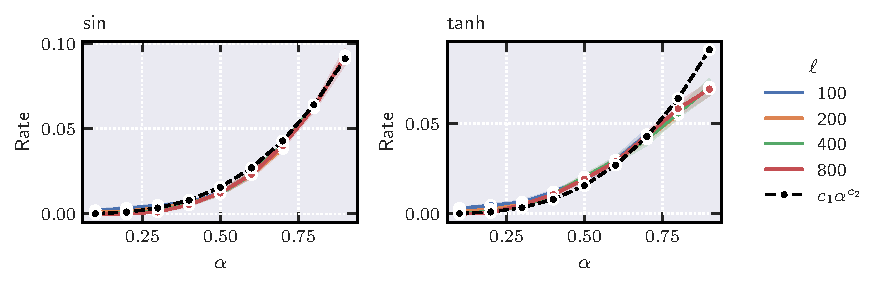
\includegraphics[width=0.8\linewidth]{figures/rate_vs_gain.pdf}
    \caption{Explosion rate of the log norm of the gradients at initialization for an MLP model with
orthogonal weights and batch normalization, for sin and tanh nonlinearities measured for a $1000$
layer deep model at layers $\ell$ as a function of gain $\alpha$. The black trace shows the fitted function $c_1 \alpha^c_2$. Traces are averaged over $10$ independent runs, with the shades showing the $95\%$ confidence interval.}
    \label{grad:fig:rate_vs_gain}
\end{figure}

This reduces the problem to picking the exponent such that the sum stays bounded. We show how the behaviour of the explosion rate at the early layers, for various models, is impacted by the exponent in Figure~\ref{grad:fig:rate_vs_exponent}. Note that for several exponent values, we able to reduce the exponential explosion rate and obtain trainable models, which we show in Section~\ref{grad:sec:other_experiments}.

\begin{figure}[ht]
    \centering
    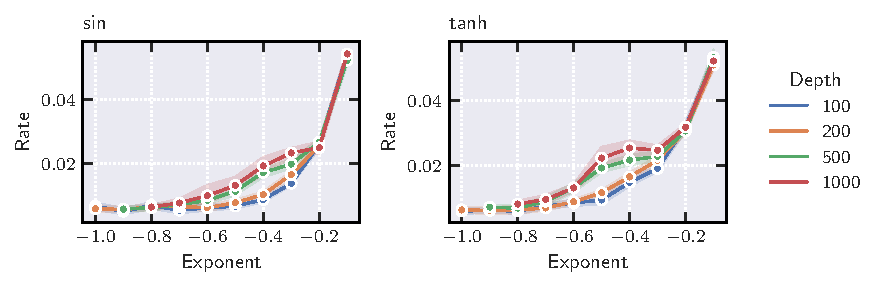
\includegraphics[width=0.8\linewidth]{figures/rate_vs_exponent.pdf}
    \caption{Explosion rate of the log norm of the gradients at initialization for an MLP model with orthogonal weights and batch normalization, for sin and tanh nonlinearities at depths $100, 200, 500, 1000$ as a function of the gain exponent. Traces are averaged over $10$ independent runs, where the shade shows the $95\%$ confidence interval. Rate is measured at $\ell=10$ to avoid the any transient effects of the function}
    \label{grad:fig:rate_vs_exponent}
\end{figure}

\section{Implicit orthogonality during training}
\label{grad:sec:implicity_orthogonality}
In this section, we provide empirical evidence that our architecture during training maintains orthogonality across depths, while maintaining bounded gradients. Figure~\ref{grad:fig:ortho_during_training} shows the evolution of the isometry gap of the weight matrices $W_\ell$ during training, for models at different depths and different nonlinearities. In order to show that these weights are updated gradient descent, we also show the evolution of the norm of the loss gradients with regards to matrices $W_\ell$ in Figure~\ref{grad:fig:gradient_during_training}. 

These experiments are performed on an MLP with orthogonal weight matrices and batch normalization, with sin and tanh activations. The width is set to $100$, batch size $100$ and learning rate $0.001$. The gain exponent is set to a fixed value for all experiments. The measurements are performed on a single batch of size $100$ from CIFAR10, after each epoch of training on the same dataset. 

\begin{figure}[htp!]
    \centering
    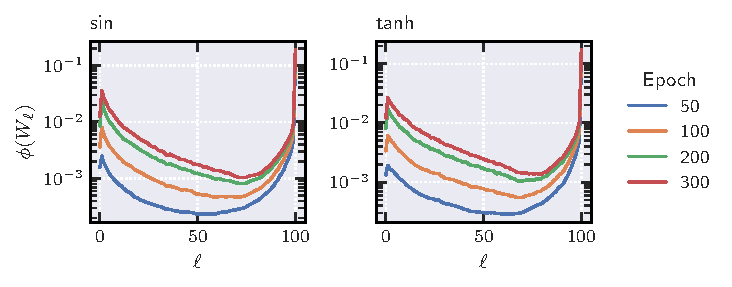
\includegraphics[width=0.8\linewidth]{figures/weight_isogap_during_training_100.pdf}
    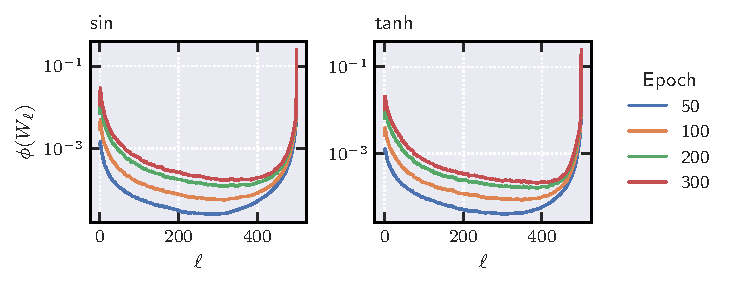
\includegraphics[width=0.8\linewidth]{figures/weight_isogap_during_training_500.pdf}
    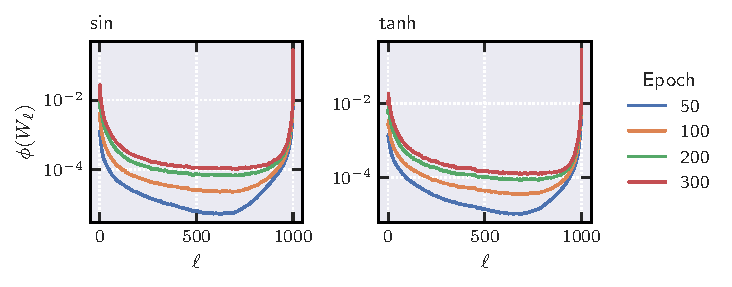
\includegraphics[width=0.8\linewidth]{figures/weight_isogap_during_training_1000.pdf}
    \caption{Contrasting the isometry gap of weight matrices during training for MLPs of depth $100$ (top), $500$ (middle), $1000$ (bottom). The middle layers become increasingly more orthogonal with depth, while maintaining a small isometry gap. During training, the isometry gap also remains low, suggesting the matrices remain close to being orthogonal.}
    \label{grad:fig:ortho_during_training}
\end{figure}

\begin{figure}[htp!]
    \centering
    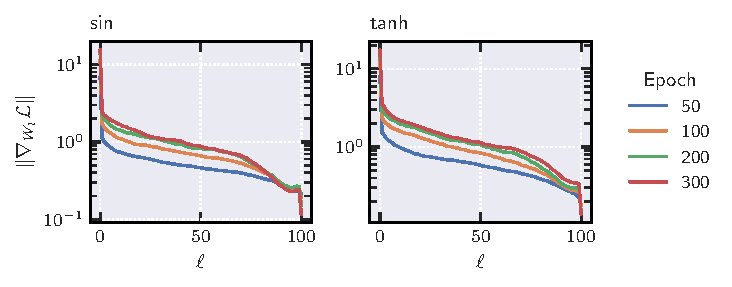
\includegraphics[width=0.8\linewidth]{figures/gradient_during_training_100.pdf}
    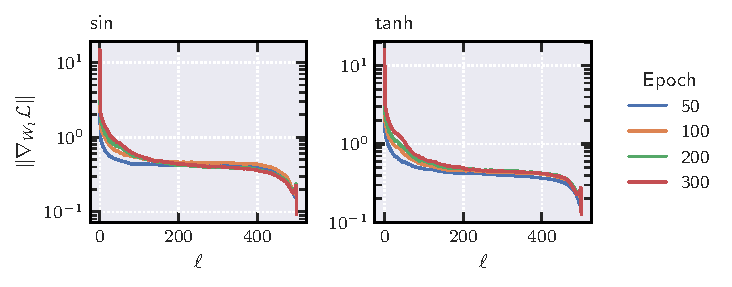
\includegraphics[width=0.8\linewidth]{figures/gradient_during_training_500.pdf}
    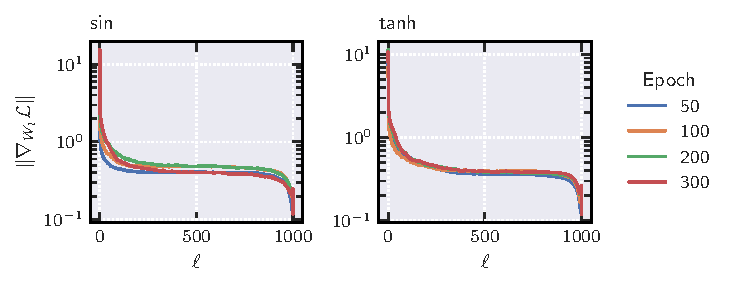
\includegraphics[width=0.8\linewidth]{figures/gradient_during_training_1000.pdf}
    \caption{Contrasting the Frobenius norm of the gradients of the loss with respect to the weights during training for MLPs of depth $100$ (top), $500$ (middle), $1000$ (bottom). The gradients do not vanish during training and across different depths for all layers, suggesting that the orthogonality evidenced in Figure~\ref{grad:fig:ortho_during_training} is not due to the weights not being updated during SGD.}
    \label{grad:fig:gradient_during_training}
\end{figure}


\section{Other experiments}
\label{grad:sec:other_experiments}
In this section we provide the train and test accuracies of deep MLPs on 4 popular image datasets, namely MNIST, FashionMNIST, CIFAR10, CIFAR100. Hyperparameters and measurements procedure are described in Section~\ref{grad:sec:experiments}.

\subsection*{Supplementary train and test results on MNIST, FashionMNIST, CIFAR10, CIFAR100}

\begin{figure}[ht]
    \centering
    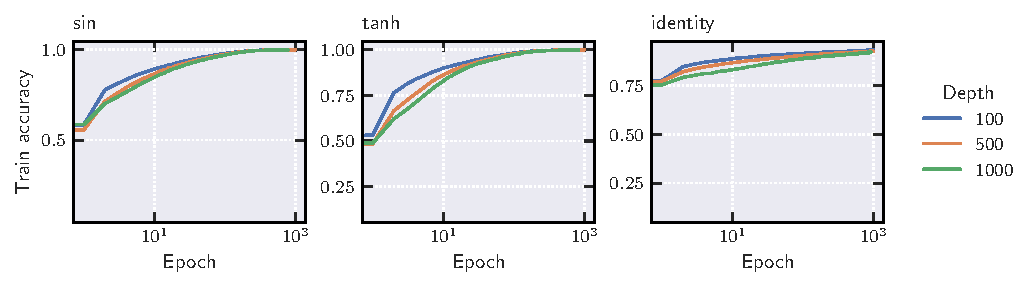
\includegraphics[width=1.0\linewidth]{figures/train_MNIST.pdf}
    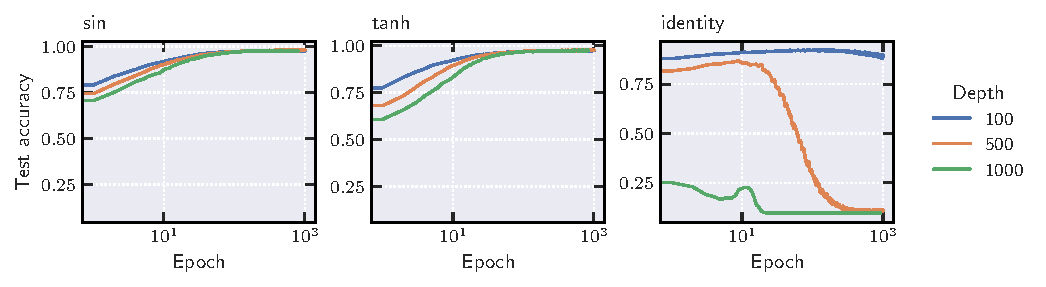
\includegraphics[width=1.0\linewidth]{figures/test_MNIST.pdf}
    \caption{Contrasting the train and test accuracy of MLPs with gained sin, tanh and identity activations on MNIST. The identity activation performs much worse than the nonlinearities, indicating the fact that the sin and tanh networks are not operating in the linear regime. The network is trained with vanilla SGD and the hyperparameters are width $100$, batch size $100$, learning rate $0.001$.}
    \label{grad:fig:mnist}
\end{figure}

\begin{figure}[ht]
    \centering
    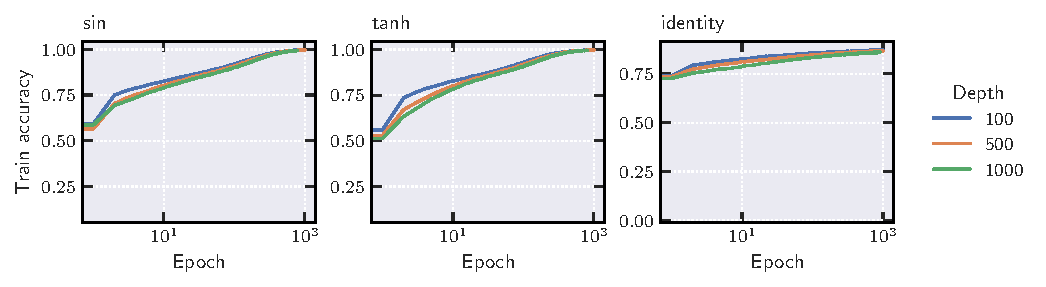
\includegraphics[width=1.0\linewidth]{figures/train_FashionMNIST.pdf}
    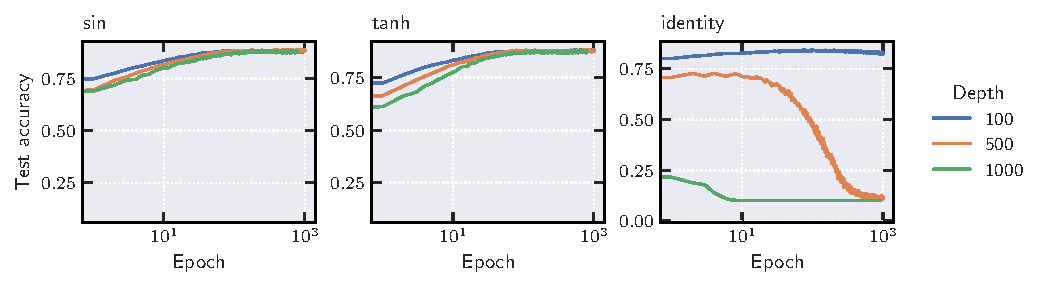
\includegraphics[width=1.0\linewidth]{figures/test_FashionMNIST.pdf}
    \caption{Contrasting the train and test accuracy of MLPs with gained sin, tanh and identity activations on FashionMNIST. The identity activation performs much worse than the nonlinearities, indicating the fact that the sin and tanh networks are not operating in the linear regime. The networks are trained with vanilla SGD and the hyperparameters are width $100$, batch size $100$, learning rate $0.001$.}
    \label{grad:fig:fashionmnist}
\end{figure}

\begin{figure}[ht]
    \centering
    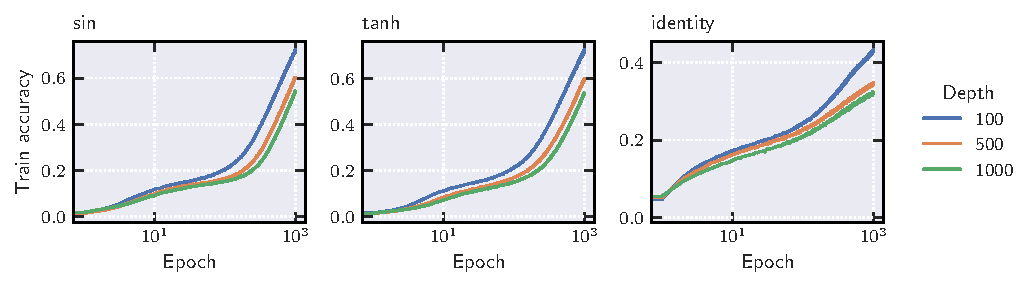
\includegraphics[width=1.0\linewidth]{figures/train_CIFAR100.pdf}
    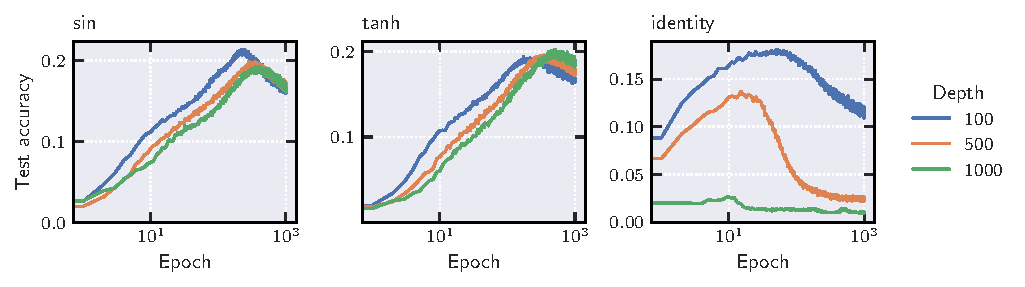
\includegraphics[width=1.0\linewidth]{figures/test_CIFAR100.pdf}
    \caption{Contrasting the train and test accuracy of MLPs with gained sin, tanh and identity activations on CIFAR100. The identity activation performs much worse than the nonlinearities, indicating the fact that the sin and tanh networks are not operating in the linear regime. The networks are trained with vanilla SGD and the hyperparameters are width $100$, batch size $100$, learning rate $0.001$.}
    \label{grad:fig:cifar100}
\end{figure}

\begin{figure}[ht]
    \centering
    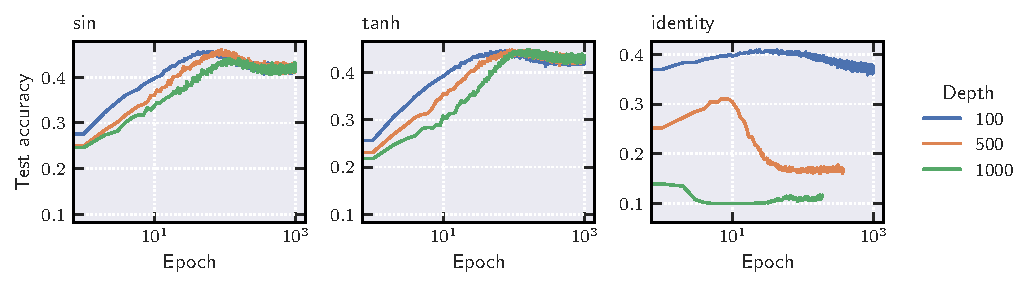
\includegraphics[width=1.0\linewidth]{figures/test_CIFAR10.pdf}
    \caption{Contrasting the train test accuracy of MLPs with gained sin, tanh and identity activations on CIFAR10. The identity activation performs much worse than the nonlinearities, indicating the fact that the sin and tanh networks are not operating in the linear regime. The networks are trained with vanilla SGD and the hyperparameters are width $100$, batch size $100$, learning rate $0.001$.}
    \label{grad:fig:cifar10_test}
\end{figure}

\subsection*{Supplemental figures}
We present empirical results in Figure~\ref{grad:fig:degenerate_input} showing that degenerate input batches are a hard constraint for orthogonalization without gradient explosion. For MLPs with different depths, we show that by repeating samples in a batch of size $10$ we get an exponential gradient explosion, which is unavoidable theoretically.



Furthermore, we show how non-linearities affect the gradient explosion rate in Figure~\ref{grad:fig:nonlinear_contrast}. Using standard batch normalization and fully connected layers from PyTorch we show that non-linearities maintain a large isometry gap. This is a critical issue for our theoretical framework, since we take advantage of the fact that the identity activation achieves perfect orthogonality in order to prove that the gradients remain bounded in depth.
\begin{figure}[ht]
    \centering
    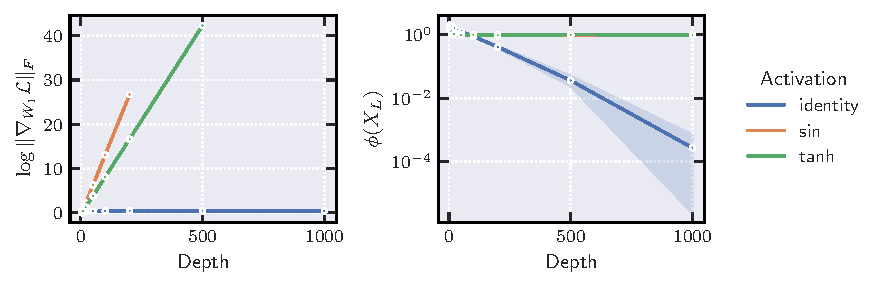
\includegraphics[width=0.9\linewidth]{figures/log_nonlinearities.pdf}
    \vspace{-.4cm}
    \caption{Left: average log-norm of gradients (log-scale y-axis) at the first layer for networks with different depths, evaluted on CIFAR10. Right: Isometry gap (log-scale y-axis) at the last layer for networks with different depths, evaluted on CIFAR10. The MLP is initialized with orthogonal weights and batch normalization, with standard modules, with $\sin, \tanh, \text{identity}$ non-linearities. After stabilizing the isometry gap, the non-linearities have an exponential gradient explosion.
    }
    \label{grad:fig:nonlinear_contrast} 
\end{figure}

\subsection*{Influence of mean reduction on the gradient bound}
In this section, we compare whether adding mean reduction and the additional factor of $\frac1n$ in the denominator of the batch normalization module influences our gradient bound. As expected, we show in Figure~\ref{grad:fig:mean_reduction} that in both cases, for the identity activation, the result remains similar, with the gradients remaining bounded in depth. 
\begin{figure}[ht!]
    \centering
    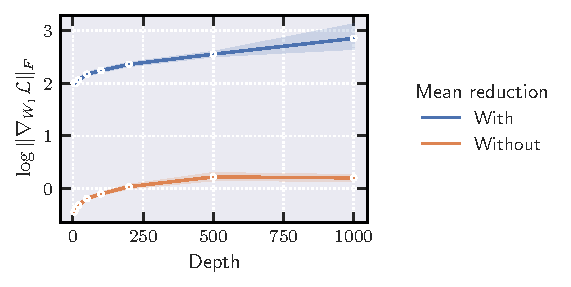
\includegraphics[width=0.6\linewidth]{figures/log_mean_reduction.pdf}
    \vspace{-.4cm}
    \caption{Comparing the gradient explosion rate in networks with standard batch normalization (blue) and networks with the simplified batch normalization operator from our theoretical framework (orange). Notice that the 2 traces are similar in terms of gradient explosion. Traces are averaged over $10$ runs with the shaded regions showing the $95\%$ confidence interval. Samples are from CIFAR10.
    }
    \label{grad:fig:mean_reduction} 
\end{figure}

% \section{High probability log-gradient bound}
% \begin{theorem}
% In the same conditions as Theorem~\ref{grad:thm:explosion_appendix}, it there is constant $C$ such that:
% $$
% \Pr\Big(\log\|\nabla_{W_\ell}\mathcal{L}\|_{op}\ge  C  \log(1/\delta) d^{6}(\psi(X^0)^3+1)\Big) \le 2\delta 
% $$
% for any $\delta \in(0,1).$
% \end{theorem}

% For example for $\delta=1/2,$ we we have $\|\nabla_{W_\ell}\mathcal{L}\|_{op}\lesssim d^{6}(\psi(X^0)^3+1)$ with at most $1/2$ probability. 
% \begin{proof}
% We follow the same proof as Theorem~\ref{grad:thm:explosion_appendix} by decomposing the log gradient to sum of log gradients of each layer. Note that Lemma~\ref{grad:lem:jacobian_bn_norm} holds deterministically, as it is valid by construction. Thus, what remains is to derive a probabilistic version of Lemma~\ref{grad:lem:jacobian_log_norm_bound}. We start from \eqref{grad:eqn:op_bound} which holds deterministically, to arrive at a probabilistic bound:
% \begin{align}
% \sum_{k = 1}^L \log \norm{J_{\BN}(H^k)} \le S (d\psi(X^0)) + 2\sum_{\ell=S+1}^L \sqrt{d\psi(X^\ell)}, \qquad S:= \min\left\{\ell: \psi(X^\ell)\le \frac{1}{16d^2}\right\}
% \end{align}
% We derive a probabilistic bound for each term.
% \newcommand{\Event}{\mathcal{E}}
% \paragraph{First term.}
% Based on Lemma~\ref{grad:lem:hitting_layer} we have $E [S] \lesssim d^4 \psi(X^0)^2.$ Thus, there is $C_0$ such that $$\exists C_0: E [S] \le \frac{C_0}{2} d^4 \psi(X^0)^2 .$$ Thus, by Markov inequality we have 
% $$P (S\ge B) \le \frac{\E[S]}{B } \le \frac12, \qquad B:=  C_0 d^4 \psi(X^0)^2. $$ 

% First, we discretize the layers into blocks of size $B$, where $B$ is defined above. With a slight abuse of notation, define $B_i$ as the end of the $i$th block of size $B$, and let $E_i$ be the event $E_i = \{\psi(X_{B_i}) > \frac{1}{16d^2}\}$, which is the event of failure for $\psi$ to drop below the threshold of $\frac{1}{16d^2}$ after the last layer from block $i$.

% By the inequality established above, we know that in each block, $\psi$ can either fall below the threshold, or stay above, with probability at most $1/2$. Moreover, knowing that $\psi$ is non-increasing, we know that $P(E_i | E_{<i}) \leq 1/2$.

% Thus, by the non-increasing property of $\psi$, the probability of failure after $k$ blocks of size $B$ is at most the probability that $\psi$ did not fall below the threshold in any of the $k$ successive blocks:

% \begin{align}
%     P(E_k) &\leq P(E_1 \wedge \dots \wedge E_{k-1}) \\
%     &= P(E_1) P(E_2 | E_1) \dots P(E_{k} | E_{k-1} \dots E_1) \\
%     &\leq \left(\frac{1}{2}\right)^k
% \end{align}

% Thus, we obtain the probability:
% \begin{align}
%     P(S \geq kB) = P(S \geq k C_0 d^4 \psi(X_0)^2) \leq 2^{-k}
% \end{align}

% Thus, connecting back to gradients, we obtain:
% \begin{align}
%     \Pr\Big(\sum_{\ell=0}^S \|J_{\BN}(H^\ell)\|_{op} \ge k C_0 d^5 \psi(X^0)^3 \Big)\le 2^{-k}.
% \end{align}

% \paragraph{Second term} Starting from~\eqref{grad:eqn:after_thresh}, we have 
% $$
% \ell \ge S \implies \Pr\Big\{\psi(X^{\ell+1})\ge (1-1/4d^2)\psi(X^\ell)\Big\} \le 1- \frac{1}{4d^2}
% $$
% Let $E_\ell$ denote the event that $\psi(X^{\ell+1})$ does not decrease by $1-1/4d^2$ compared to its previous layer:
% $E_\ell = \1\Big\{\psi(X^{\ell+1})\ge (1-1/4d^2)\psi(X^\ell)\Big\}.$
% Due to the non-increasing property of $\psi$, we know that $\Pr(E_\ell) = \Pr(E_\ell | E_{\ell-1})$. Repeating this for $s$ steps, we obtain:

% \begin{align}
%     \ell \ge S \implies \Pr\Big\{\psi(X^{\ell+s})\ge (1-1/4d^2)\psi(X^\ell)\Big\} =
%     \prod_{i=\ell}^{\ell+s-1} \Pr\{ E_{i+1} | \bar E_{i} \} \leq (1 - \frac{1}{4d^2})^s
% \end{align}

% Inspired by this, consider the sequence $\ell_0, \ell_1, \dots$ defined as 
% $$
% \ell_0 = S, \qquad \ell_{k} = \ell_{k-1} + 4 c k d^2
% $$
% Thus, we get:
% $$
% \Pr\Big\{\psi(X^{\ell_{k+1}})\ge (1-\frac{1}{4d^2})\psi(X^{\ell_{k}})\Big\} \le (1- \frac{1}{4d^2})^{4 c k d^2} \le e^{-ck}
% $$
% Thus, we have the union bound 
% \begin{align*}
% \Pr\Big\{\bigvee_{k=0}^\infty \psi(X^{\ell_{k+1}})\ge (1-\frac{1}{4d^2})\psi(X^{\ell_k}) \Big\} \le \sum_{k=1}^\infty e^{-ck} = \frac{e^{-c}}{1-e^{-c}}\\
% \implies \Pr\Big\{\underbrace{\bigwedge_{k=0}^\infty \psi(X^{\ell_{k+1}})\le (1-\frac{1}{4d^2})\psi(X^{\ell_k}) }_{Q:=}\Big\} \ge 1- \frac{e^{-c}}{1-e^{-c}}= \frac{1-2e^{-c}}{1-e^{-c}}
% \end{align*}
% Note that in the event that $Q$ holds, we can the isometry gaps in each $[\ell_{k-1},\ell_k]$ interval as:
% $$
% Q \implies \psi(X_\ell) \le \frac{1}{16d}(1-\frac{1}{4d^2})^{k-1} \text{ for all } \ell \in [\ell_{k-1},\ell_{k})
% $$
% We can upper bound $\sum_{\ell=S+1}^\infty \sqrt{d \psi(X^\ell)}$ by using the numbers of items and upper bound on each block. Thus, assuming for all $k$  we have  $\psi(X^{\ell_{k+1}})\le (1-\frac{1}{4d^2})\psi(X^{\ell_k}),$ we can derive
% \begin{align*}
% Q \implies \sum_{\ell=S+1}^\infty \sqrt{d\psi(X_\ell)} &\le \sum_{k=1}^\infty (\ell_{k}-\ell_{k-1})\sqrt{d \frac{1}{16d} (1-\frac{1}{4d^2})^{k}}\\
% & = cd^2 \sum_{k=1}^\infty k (1-\frac{1}{4d^2})^{k/2} \\
% &\le c d^2 \sum_{k=1}^\infty k(1-\frac{1}{8d^2})^k && \text{using $(1+x)^{1/2}\le 1+x/2$}\\
% &= cd^2 \frac{1-8/d^2}{(1/8d^2)^2}   && \text{using $\sum_{k=1}^\infty k\alpha^k = \alpha/(1-\alpha)^2.$}\\
% &\le 64 c d^6 
% \end{align*}
% Thus we have:
% $$
% \Pr\left(\sum_{\ell=S+1}^\infty \sqrt{d\psi(X_\ell)} \le 64 c d^6 \right) \ge \Pr\Big\{Q \Big\} \ge \frac{1-2e^{-c}}{1-e^{-c}}
% $$
% which yields 
% $$
% \Pr\left(\sum_{\ell=S+1}^\infty \log\|J_{BN}(H^\ell)\|_{op}  \ge 64 c d^6 \right) \le \Pr(\overline Q)= \frac{e^{-c}}{1-e^{-c}}
% $$
% Combining first and second term bounds for the Jacobian log-norms we have
% \begin{align}
% \Pr\Big(\sum_{l=\ell}^S \log\|J_{\BN}(H^l)\|_{op} > k C_0 d^5\psi(X^0)^3\Big) &\le 2^{-k} \\
% P\left(\sum_{\ell=S+1}^\infty \log\|J_{\BN}(H^l)\|_{op} \ge 64 cd^{6}\right) &\le \frac{e^{-c}}{1-e^{-c}}
% \end{align}
% And thus we have 
% $$
% \Pr\Big(\sum_{l=\ell}^L\log\|J_{BN}(H^l)\|_{op} \ge k C_0 d^5\psi(X^0)^3 + 64 cd^{6}\Big) \le 2^{-k} + \frac{e^{-c}}{1-e^{-c}}
% $$
% Thus, we can find $C$ such that 
% $$
% \Pr\Big(\log\|\nabla_{W_\ell}\mathcal{L}\|_{op}\ge k C  d^{6}(\psi(X^0)^3+1)\Big) \le 2^{-k+1}
% $$
% We can finish the proof by defining $\delta = 2^{-k}$ and change of variables $k = \log(1/\delta).$
% \end{proof}

% \section{Gradients in Residual networks}
% \begin{figure}[htp]
%     \centering
%     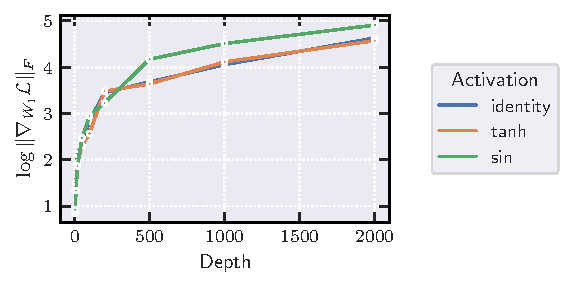
\includegraphics{figures/rebuttal_residual.pdf}
%     \caption{Logarithmic plot for the gradient norm of the first layer for residual networks with batch normalization initialized with Gaussian weights at different depths, evaluated on CIFAR10. The traces show that the gradients do not remain bounded in depth for different activations.}
%     \label{grad:fig:residuals}
% \end{figure}

